\documentclass[12pt, letterpaper]{article}
\usepackage[margin=1in]{geometry}
\usepackage[T1]{fontenc}
\usepackage{lmodern}
\usepackage{cmap}
\usepackage[utf8]{inputenc}
\usepackage{amsmath, amssymb, amsthm}
\usepackage{mathtools}
\usepackage{enumitem}
\usepackage{booktabs}
\usepackage{xcolor}
\usepackage{titlesec}
\usepackage{parskip}
\usepackage{hyperref}
\usepackage{fancyhdr}
\usepackage{tcolorbox}
\usepackage{graphicx}
\usepackage{caption}
\tcbuselibrary{skins, breakable}

\definecolor{darkblue}{RGB}{15,55,115}
\definecolor{midblue}{RGB}{30,100,180}
\definecolor{theorybg}{RGB}{245,250,255}
\definecolor{questionbg}{RGB}{255,252,240}
\definecolor{evencolor}{RGB}{60,0,100}

\hypersetup{colorlinks=true,linkcolor=darkblue,urlcolor=midblue,
  pdftitle={Ljungqvist \& Sargent --- Recursive Macroeconomic Theory --- Complete Solutions, Chapter 6}}

\setlength{\headheight}{14pt}
\pagestyle{fancy}
\fancyhf{}
\renewcommand{\headrulewidth}{0.4pt}
\fancyhead[L]{\small\textcolor{darkblue}{\textit{Ljungqvist \& Sargent --- Recursive Macroeconomic Theory}}}
\fancyhead[R]{\small\textcolor{darkblue}{\thepage}}
\fancyfoot[C]{\small\textcolor{gray}{Complete Solutions --- Chapter 6}}

\titleformat{\section}[block]
  {\large\bfseries\color{darkblue}}{}{0pt}{}
  [\vspace{2pt}\color{darkblue}\rule{\textwidth}{1.5pt}\vspace{4pt}]

\titleformat{\subsection}[block]
  {\normalsize\bfseries\color{midblue}}{}{0pt}{}
  [\vspace{1pt}\color{midblue}\rule{0.5\textwidth}{0.8pt}\vspace{3pt}]

\tcbset{
  theorybox/.style={
    enhanced,breakable,colback=theorybg,colframe=darkblue,
    fonttitle=\bfseries\small\color{darkblue},boxrule=0.5pt,arc=3pt,
    left=6pt,right=6pt,top=4pt,bottom=4pt,title={Key Theory},
  },
  questionbox/.style={
    enhanced,breakable,colback=questionbg,colframe=gray!60,
    fonttitle=\bfseries\small\color{gray!60!black},boxrule=0.4pt,arc=2pt,
    left=6pt,right=6pt,top=4pt,bottom=4pt,title={\textit{Question}},
  },
  oddbox/.style={
    enhanced,breakable,colback=white,colframe=darkblue,
    attach boxed title to top left={yshift=-2mm,xshift=6mm},
    boxed title style={colback=darkblue,colframe=darkblue,arc=2pt,
      boxrule=0pt,left=6pt,right=6pt,top=3pt,bottom=3pt},
    fonttitle=\bfseries\large\color{white},
    boxrule=0.8pt,arc=3pt,
    left=8pt,right=8pt,top=10pt,bottom=6pt,
  },
  evenbox/.style={
    enhanced,breakable,colback=white,colframe=evencolor,
    attach boxed title to top left={yshift=-2mm,xshift=6mm},
    boxed title style={colback=evencolor,colframe=evencolor,arc=2pt,
      boxrule=0pt,left=6pt,right=6pt,top=3pt,bottom=3pt},
    fonttitle=\bfseries\large\color{white},
    boxrule=0.8pt,arc=3pt,
    left=8pt,right=8pt,top=10pt,bottom=6pt,
  },
  databox/.style={
    enhanced,breakable,colback=gray!8,colframe=gray!55,
    fonttitle=\bfseries\small\color{gray!60!black},boxrule=0.4pt,arc=2pt,
    left=6pt,right=6pt,top=4pt,bottom=4pt,title={Numerical exercise --- see the companion code},
  },
  trapbox/.style={
    enhanced,breakable,colback=red!4,colframe=red!45!black,
    fonttitle=\bfseries\small\color{white},boxrule=0.4pt,arc=2pt,
    coltitle=white,
    left=6pt,right=6pt,top=4pt,bottom=4pt,title={Where this goes wrong},
  },
}

\newcommand{\pd}[2]{\dfrac{\partial #1}{\partial #2}}
\newcommand{\dd}[2]{\dfrac{d #1}{d #2}}
\newcommand{\MRS}{\mathrm{MRS}}
\newcommand{\MRT}{\mathrm{MRT}}
\newcommand{\MU}{\mathrm{MU}}
\newcommand{\Var}{\mathrm{Var}}
\newcommand{\Cov}{\mathrm{Cov}}
\newcommand{\E}{\mathrm{E}}
\newcommand{\MPK}{\mathrm{MPK}}
\newcommand{\MPL}{\mathrm{MPL}}
\newcommand{\wb}{\bar w}
\newcommand{\Gint}[1]{\int_{#1}^{B}(w'-#1)\,dF(w')}

\setlist[enumerate,1]{label=(\alph*),itemsep=6pt,parsep=2pt}
\setlist[enumerate,2]{label=(\roman*),itemsep=3pt}

\begin{document}

%======================================================================
% TITLE PAGE
%======================================================================
\begin{titlepage}
\centering
\vspace*{2.5cm}
{\Huge\bfseries\color{darkblue} Recursive Macroeconomic Theory\par}
\vspace{6pt}
{\large Lars Ljungqvist and Thomas J.\ Sargent (4th ed., 2018)\par}
\vspace{1.4cm}
{\LARGE\bfseries Complete Solutions\par}
\vspace{6pt}
{\LARGE\bfseries Chapter 6 --- Search and Unemployment\par}
\vspace{1.2cm}
{\large All twenty-seven end-of-chapter exercises, 6.1--6.27 (pp.~204--222)\par}
\vspace{2cm}

\begin{tcolorbox}[theorybox,title={What is in this file},width=0.86\textwidth]
\small
Each exercise has a short restatement of the question (page number given; see the book for the full
wording), a step-by-step solution with no skipped algebra, and a verification. Numerical answers
come from the companion notebook \texttt{Resolucao/ljungqvist\_sargent/ls\_ch06.ipynb}, which has one
section per exercise and checks every number by an independent route --- the reservation-wage
equation against value-function iteration on the whole function, exact evaluation of cutoff rules,
exhaustive policy enumeration, Howard iteration, or Monte Carlo --- and aborts on any mismatch. The
two exercises that ask for Matlab (6.18, 6.25) are done in Python.

\smallskip
Where the book gives no numbers we choose standard ones and state them. Exercises are grouped by
\textbf{topic}, not by number. Blue boxes are odd-numbered exercises, purple boxes even.

\smallskip
Ljungqvist--Sargent is supplementary reading and lies outside the course syllabus; this file is
for depth, not for the exam.
\end{tcolorbox}

\vfill
{\small MPE Insper --- Macroeconomia I --- 2026, 3\textordmasculine{} trimestre\par}
\end{titlepage}

\tableofcontents
\newpage

%======================================================================
\section{Chapter 6 \quad Search and Unemployment}
%======================================================================

\begin{tcolorbox}[theorybox,title={Chapter 6 Overview}]
\textbf{McCall's model} (section 6.3). An unemployed worker draws one offer $w\sim F$, $F(0)=0$, $F(B)=1$,
each period; accepting pays $w$ forever, rejecting pays $c$ today and a fresh draw tomorrow:
\[
v(w)=\max\Big\{\frac{w}{1-\beta},\;c+\beta\int_0^Bv(w')\,dF(w')\Big\}. \tag{6.3.1}
\]
Accepting is worth more for higher $w$, rejecting is a constant $Q$, so the policy is a
\emph{reservation wage} $\wb=(1-\beta)Q$, which solves
\[
\wb-c=\frac{\beta}{1-\beta}\Gint{\wb}\equiv h(\wb) \tag{6.3.3}
\]
or, after integrating by parts, $\wb-c=\beta(Ew-c)+\beta\int_0^{\wb}F(w')\,dw'$ (6.3.5).

\smallskip
\textbf{The reduction used throughout.} If rejecting is worth $Q$ and accepting is worth
$\wb$-increasing $a(w)$ with $a(\wb)=Q$, then $\int\max\{a(w'),Q\}dF=Q+\int_{\wb}[a(w')-a(\wb)]dF$. With
$a(w)=w/(1-\beta)$ this is $Q+\frac1{1-\beta}\Gint{\wb}$. We write
$G_F(x)\equiv\int_x^B(w'-x)\,dF(w')=\int_x^B[1-F(w')]\,dw'$ for this option-value integral.

\smallskip
\textbf{Mean-preserving spreads} (section 6.2). $F_1$ is an MPS of $F_2$ if (i) the means are equal and
(iii) $\int_0^y[F_1-F_2]\,d\theta\ge0$ for all $y$. Because $g(s)=\int_0^sF$ enters (6.3.5), an MPS raises
$\wb$ (section 6.3.2): the worker holds an option and only the right tail matters.

\smallskip
\textbf{Also used:} quits and firing (6.3.3, 6.3.5), waiting times $1/(1-F(\wb))$ (6.3.4), Neal's career
choice model (section 6.5, Bellman equation (6.5.1), cutoffs $\bar\theta$, $\bar\epsilon$), and Howard's
policy improvement (chapter 3).
\end{tcolorbox}

%======================================================================
\subsection{Variations on McCall's Bellman Equation}
%======================================================================

%------- 6.1 -------
\begin{tcolorbox}[oddbox,title={Exercise 6.1 \quad Being Unemployed with a Chance of an Offer}]
\begin{tcolorbox}[questionbox]
(p.~204) Each period, with probability $\phi\in(0,1)$ the unemployed worker gets no offer (an offer of
zero forever); with probability $1-\phi$ she draws $w\sim F$. Income $y_t=w$ employed, $c$ unemployed; jobs
last forever. Write the Bellman equation for $v(w)$, the value of an unemployed worker with offer $w$ in
hand.
\end{tcolorbox}

\textbf{Solution:}

\emph{Bellman equation.} Next period's offer is $0$ with probability $\phi$ and a draw from $F$ with
probability $1-\phi$:
\[
\boxed{v(w)=\max\Big\{\frac{w}{1-\beta},\;c+\beta\Big[\phi\,v(0)+(1-\phi)\int_0^Bv(w')\,dF(w')\Big]\Big\}}
\]

\emph{Reservation wage.} The second argument, $Q$, does not depend on $w$; the first rises with $w$. So
$v(w)=\max\{w/(1-\beta),Q\}$ and $\wb=(1-\beta)Q$. The zero offer is rejected whenever $Q>0$ (true for
$c>0$), so $v(0)=Q$. Using the reduction of the overview,
$\int v\,dF=Q+\frac{1}{1-\beta}G_F(\wb)$, hence
\[
Q=c+\beta\phi Q+\beta(1-\phi)\Big[Q+\frac{G_F(\wb)}{1-\beta}\Big]
\;\Longrightarrow\;(1-\beta)Q=c+\frac{\beta(1-\phi)}{1-\beta}G_F(\wb),
\]
and with $(1-\beta)Q=\wb$:
\[
\boxed{\wb-c=\frac{\beta(1-\phi)}{1-\beta}\int_{\wb}^B(w'-\wb)\,dF(w')}
\]
This is (6.3.3) with the option value scaled by $1-\phi$. The right side falls with $\phi$ and the left side
rises with $\wb$, so a higher chance of no offer lowers the reservation wage. The exit probability is
$(1-\phi)[1-F(\wb)]$ per period and the mean duration is its inverse (section 6.3.4).

\begin{tcolorbox}[databox]
$F$ uniform on $[0,10]$ (200-point grid), $c=1$, $\beta=.95$:
\begin{center}
\begin{tabular}{@{}lccc@{}}
\toprule
$\phi$ & $0$ & $.3$ & $.6$\\
\midrule
$\wb$ (equation $=$ VFI with an explicit zero offer) & $7.4037$ & $6.9970$ & $6.2744$\\
mean duration $1/[(1-\phi)(1-F(\wb))]$ & $3.846$ & $4.762$ & $6.667$\\
simulated (20\,000 spells) & $3.822$ & $4.764$ & $6.725$\\
\bottomrule
\end{tabular}
\end{center}
\end{tcolorbox}
\end{tcolorbox}

%------- 6.2 -------
\begin{tcolorbox}[evenbox,title={Exercise 6.2 \quad Two Offers per Period}]
\begin{tcolorbox}[questionbox]
(pp.~206--207) The unemployed worker draws \emph{two} i.i.d.\ offers from $F$ each period; $v(w)$ is the
value with best offer $w$ in hand. (a) Bellman equation. (b) Prove that the reservation wage is higher
than with one offer per period.
\end{tcolorbox}

\textbf{Solution:}

\textbf{(a)} The best of two independent draws has c.d.f.\ $\Pr\{\max(w_1,w_2)\le w\}=F(w)^2$:
\[
\boxed{v(w)=\max\Big\{\frac{w}{1-\beta},\;c+\beta\int_0^Bv(w')\,dF^2(w')\Big\}}
\]
As in McCall, $\wb_2=(1-\beta)Q_2$ solves $\wb_2-c=h_2(\wb_2)$ with
$h_k(x)\equiv\frac{\beta}{1-\beta}\int_x^B(w'-x)\,dF^k(w')$.

\textbf{(b)} Integrating by parts,
$\int_x^B(w'-x)\,dF^k(w')=\big[(w'-x)(F^k(w')-1)\big]_x^B+\int_x^B[1-F^k(w')]\,dw'=\int_x^B[1-F^k(w')]\,dw'$, so
\[
h_2(x)-h_1(x)=\frac{\beta}{1-\beta}\int_x^BF(w')[1-F(w')]\,dw'\;\ge0,
\]
strictly for $x<B$ whenever $0<F<1$ on a set of positive length in $(x,B)$ (true for any nondegenerate
$F$ once $x$ lies below the top of the support). Let $\psi_k(x)=x-c-h_k(x)$. Each $\psi_k$ is strictly
increasing ($h_k'=-\frac{\beta}{1-\beta}[1-F^k]\le0$), and $\wb_k$ is its root. With $c<B$ we have $\wb_1<B$ and
\[
\psi_2(\wb_1)=\underbrace{\psi_1(\wb_1)}_{=0}-[h_2(\wb_1)-h_1(\wb_1)]<0
\;\Longrightarrow\;\boxed{\wb_2>\wb_1}.
\]
A second offer is a first-order-dominating improvement of the offer distribution: every draw is at least
as good, so waiting is worth more and the worker becomes choosier. (If $c\ge B$ nobody ever accepts and
both "reservation wages" equal $c$.)

\begin{tcolorbox}[databox]
$F$ uniform on $[0,10]$, $\beta=.95$. $\wb_1$ vs.\ $\wb_2$: $c=0$: $7.2395<7.8866$; $c=1$: $7.4037<8.0119$;
$c=3$: $7.7613<8.2824$; $c=6$: $8.4079<8.7674$. $\wb_2$ is reproduced by VFI on the \emph{pair} of offers
$(w_1,w_2)$, which never uses $F^2$, and the best grid cutoff (exact policy evaluation) is the first
grid point above $\wb_2$.
\end{tcolorbox}
\end{tcolorbox}

%------- 6.3 -------
\begin{tcolorbox}[oddbox,title={Exercise 6.3 \quad A Random Number of Offers per Period}]
\begin{tcolorbox}[questionbox]
(p.~207) Each period the worker gets $n$ offers with probability $\pi_n$, $n=1,\dots,N$, i.i.d.\ over time;
offers i.i.d.\ from $F$. Formulate the Bellman equation for $v(w)$, the value with best offer $w$ in hand.
\end{tcolorbox}

\textbf{Solution:}

Conditional on $n$ the best offer has c.d.f.\ $F^n$; unconditionally it has
$H(w)=\sum_{n=1}^N\pi_nF(w)^n$. Hence
\[
\boxed{v(w)=\max\Big\{\frac{w}{1-\beta},\;c+\beta\sum_{n=1}^N\pi_n\int_0^Bv(w')\,dF^n(w')\Big\}}
=\max\Big\{\frac{w}{1-\beta},\;c+\beta\int_0^Bv\,dH\Big\}
\]
It is McCall with offer distribution $H$, so $\wb-c=\frac{\beta}{1-\beta}\int_{\wb}^B(w'-\wb)\,dH(w')$. Since
$F^N\le H\le F$, the argument of 6.2(b) places $\wb$ between the one-offer and the $N$-offer reservation
wages.

\begin{tcolorbox}[databox]
$\pi=(.2,.5,.3)$ for $n=1,2,3$, $F$ uniform on $[0,10]$, $c=1$, $\beta=.95$: $\wb=8.0368$ (equation, VFI and
the best cutoff agree), between $7.4037$ ($n\equiv1$) and $8.3044$ ($n\equiv3$).
\end{tcolorbox}
\end{tcolorbox}

%------- 6.4 -------
\begin{tcolorbox}[evenbox,title={Exercise 6.4 \quad Cyclical Fluctuations in the Number of Job Offers}]
\begin{tcolorbox}[questionbox]
(p.~207) As in 6.3, but $n$ follows a Markov chain,
$\Pr\{n_{t+1}=m\mid n_t=n\}=\pi_{mn}$, $\sum_m\pi_{mn}=1$. (a) Bellman equation for $v(w,n)$, the value with $n$
offers this period, best $w$. (b) Show that the optimal policy is a reservation wage $\wb(n)$.
\end{tcolorbox}

\textbf{Solution:}

\textbf{(a)} Today's $n$ matters only as a predictor of tomorrow's number of offers:
\[
\boxed{v(w,n)=\max\Big\{\frac{w}{1-\beta},\;c+\beta\sum_{m=1}^N\pi_{mn}\int_0^Bv(w',m)\,dF^m(w')\Big\}}
\]
(Note the book's index order: the first subscript of $\pi_{mn}$ is \emph{next} period's state, so the
columns of $[\pi_{mn}]$ sum to one.)

\textbf{(b)} Call the second argument $Q(n)$. It depends on $n$ but not on $w$, while $w/(1-\beta)$ is strictly
increasing in $w$. So for each $n$ the worker accepts iff $w\ge\wb(n)\equiv(1-\beta)Q(n)$. The $N$ numbers
$Q(n)$ solve a finite system: by the reduction of the overview,
$\int v(w',m)\,dF^m=Q(m)+\frac1{1-\beta}\int_{\wb(m)}^B(w'-\wb(m))\,dF^m(w')$, so
\[
Q(n)=c+\beta\sum_{m}\pi_{mn}\Big[Q(m)+\frac{1}{1-\beta}\int_{(1-\beta)Q(m)}^B\big(w'-(1-\beta)Q(m)\big)\,dF^m(w')\Big],
\]
a contraction in $(Q(1),\dots,Q(N))$ with modulus $\beta$. When the chain is persistent, many offers today
forecast many offers tomorrow, raising $Q(n)$ and hence $\wb(n)$ with $n$: reservation wages are
procyclical.

\begin{tcolorbox}[databox]
$N=3$, $\Pr(m\mid n)$ with rows $(.8,.15,.05)$, $(.1,.8,.1)$, $(.05,.15,.8)$; $F$ uniform on $[0,10]$, $c=1$,
$\beta=.95$: $\wb(1),\wb(2),\wb(3)=7.7076,\ 7.9783,\ 8.1637$. VFI on the full $(w,n)$ grid gives the same numbers,
and its accept set is an upper interval in $w$ for each $n$.
\end{tcolorbox}
\end{tcolorbox}

%------- 6.5 -------
\begin{tcolorbox}[oddbox,title={Exercise 6.5 \quad Choosing the Number of Offers}]
\begin{tcolorbox}[questionbox]
(p.~208) At cost $k(n)$, increasing in $n$, the worker receives $n$ offers from $F$ this period; $n$ is chosen
at the start of the period. Income: $w$ employed and not searching, $w-k(n)$ in the first period of a job,
$c-k(n)$ when unemployed. Formulate the Bellman equation for $Q$, the value before choosing $n$.
\end{tcolorbox}

\textbf{Solution:}

Given $n$, the best offer $w$ has c.d.f.\ $F^n$. Accepting yields $w-k(n)$ today and $w$ forever after,
$\frac{w}{1-\beta}-k(n)$; rejecting yields $c-k(n)+\beta Q$. The cost is sunk in both branches, so
\[
\boxed{Q=\max_{n\ge1}\Big\{-k(n)+\int_0^B\max\Big\{\frac{w}{1-\beta},\;c+\beta Q\Big\}\,dF^n(w)\Big\}}
\]
\emph{Policy.} Given $Q$, the acceptance rule is a reservation wage $\wb=(1-\beta)(c+\beta Q)$ that does not
depend on the $n$ chosen; by stationarity the same $n^*$ is chosen every period of the spell. By the
reduction of the overview, $\int\max\{\cdot\}dF^n=c+\beta Q+\frac1{1-\beta}\int_{\wb}^B[1-F^n(w)]\,dw$, so the
gain from one more offer is
\[
\Delta(n)=\frac{1}{1-\beta}\int_{\wb}^BF(w)^n[1-F(w)]\,dw,
\]
decreasing in $n$. The optimal $n^*$ is the largest $n$ with $\Delta(n-1)\ge k(n)-k(n-1)$.

\begin{tcolorbox}[databox]
$k(n)=2n$, $F$ uniform on $[0,10]$, $c=1$, $\beta=.95$: $n^*=6$, $Q=164.8023$, $\wb=7.8781$. Iterating on $Q$ and
evaluating exactly every stationary rule "(solicit $n$, accept iff $w\ge x$)'' for $n\le15$ and every grid
$x$ give the same optimum.
\end{tcolorbox}
\end{tcolorbox}

%------- 6.7 -------
\begin{tcolorbox}[oddbox,title={Exercise 6.7 \quad Variable Labor Supply}]
\begin{tcolorbox}[questionbox]
(p.~209) Maximise $E\sum\beta^tu(y_t,l_t)$ with $y_t=c$ if unemployed and $y_t=w(1-l_t)$ if employed at $w$
(leisure $l_t\in[0,1]$). Analyse the problem; show the reservation-wage property and that hours are the
same every period.
\end{tcolorbox}

\textbf{Solution:}

Assume $u$ increasing in both arguments. An unemployed worker does not work, $l=1$. Once employed at $w$
the worker faces the same static problem every period (no savings, $w$ fixed, nothing carried over), so
\[
u^*(w)\equiv\max_{0\le l\le1}u\big(w(1-l),l\big),\qquad l_t=l^*(w)\ \text{for all }t,
\]
and hours $1-l^*(w)$ are constant over the job. The Bellman equation is
\[
\boxed{v(w)=\max\Big\{\frac{u^*(w)}{1-\beta},\;u(c,1)+\beta\int v(w')\,dF(w')\Big\}}
\]
\emph{Reservation wage.} $u^*$ is nondecreasing: for $w'>w$,
$u^*(w')\ge u\big(w'(1-l^*(w)),l^*(w)\big)\ge u\big(w(1-l^*(w)),l^*(w)\big)=u^*(w)$. The accept value is
nondecreasing in $w$ and the reject value is constant, so accept iff $w\ge\wb$ with
\[
u^*(\wb)-u(c,1)=\frac{\beta}{1-\beta}\int_{\wb}^B[u^*(w')-u^*(\wb)]\,dF(w'),
\]
(6.3.3) with wages replaced by the indirect utilities they buy. Hours can differ \emph{across} jobs
($l^*$ depends on $w$ through income and substitution effects) but not over time within a job.

\begin{tcolorbox}[databox]
$u(y,l)=2\sqrt y-1/l$, $c=1$, $F$ uniform on $[0,10]$, $\beta=.95$. $l^*(w)$ from the FOC $1/l^2=\sqrt w/\sqrt{1-l}$
agrees with direct maximisation to $10^{-5}$. $\wb=7.9348$ (equation $=$ VFI cutoff); hours $0.4992$ at
$\wb$ and $0.5219$ at $w=10$.
\end{tcolorbox}
\end{tcolorbox}

%------- 6.8 -------
\begin{tcolorbox}[evenbox,title={Exercise 6.8 \quad Wage Growth Rate and the Reservation Wage}]
\begin{tcolorbox}[questionbox]
(pp.~209--210) An accepted offer pays $w_t=\phi^tw$ after $t$ periods of tenure, $\phi>1$, $\phi\beta<1$;
unemployed get $c$. Write the Bellman equation. Argue that if $\phi_1>\phi_2$ the economy with $\phi_1$ has
the smaller reservation wage.
\end{tcolorbox}

\textbf{Solution:}

Accepting $w$ is worth $\sum_t\beta^t\phi^tw=\frac{w}{1-\beta\phi}$ (finite because $\beta\phi<1$):
\[
\boxed{v(w)=\max\Big\{\frac{w}{1-\beta\phi},\;c+\beta\int v(w')\,dF(w')\Big\}}
\]
The reservation wage satisfies $\frac{\wb}{1-\beta\phi}=Q=c+\beta\int v\,dF$, and
$\int v\,dF=Q+\frac{1}{1-\beta\phi}G_F(\wb)$. So
\[
\frac{\wb}{1-\beta\phi}=c+\frac{\beta\wb}{1-\beta\phi}+\frac{\beta G_F(\wb)}{1-\beta\phi}
\;\Longrightarrow\;
\boxed{(1-\beta)\wb=(1-\beta\phi)\,c+\beta\int_{\wb}^B(w'-\wb)\,dF(w')}
\]
Let $\Psi(\wb,\phi)=(1-\beta)\wb-(1-\beta\phi)c-\beta G_F(\wb)$. Then
$\Psi_{\wb}=1-\beta+\beta[1-F(\wb)]=1-\beta F(\wb)>0$ and $\Psi_\phi=\beta c$, so
\[
\frac{d\wb}{d\phi}=-\frac{\beta c}{1-\beta F(\wb)}<0\quad\text{for }c>0 .
\]
Hence $\phi_1>\phi_2\Rightarrow\wb(\phi_1)<\wb(\phi_2)$. Faster wage growth multiplies the value of
\emph{every} job by the same factor $1/(1-\beta\phi)$ but leaves the flow $c$ that is given up by
accepting unchanged, so waiting becomes relatively less attractive.

\emph{Caveat.} With $c=0$ the problem is homogeneous: dividing the Bellman equation by $1/(1-\beta\phi)$
shows $\wb$ is independent of $\phi$. The claim is strict only for $c>0$.

\begin{tcolorbox}[databox]
$F$ uniform on $[0,10]$, $\beta=.95$. $c=1$: $\wb=7.4037,\ 7.3403,\ 7.2780$ for $\phi=1,\ 1.02,\ 1.04$.
$c=0$: $\wb=7.2395$ for all three. Equation and VFI agree to $10^{-8}$.
\end{tcolorbox}
\end{tcolorbox}

%------- 6.12 -------
\begin{tcolorbox}[evenbox,title={Exercise 6.12 \quad Search and Financial Income}]
\begin{tcolorbox}[questionbox]
(pp.~211--212) Every agent also gets financial income $\epsilon_t$, i.i.d.\ with c.d.f.\ $G$, independent of
offers. Employed at $w$: $y_t=w+\phi\epsilon_t$, $0<\phi<1$; unemployed: $y_t=c+\epsilon_t$;
$1>\Pr\{w\ge c+(1-\phi)\epsilon\}>0$. Write the Bellman equation and show that the reservation wage
increases with the level of financial income.
\end{tcolorbox}

\textbf{Solution:}

The state is the pair $(w,\epsilon)$ observed this period. Let $\mu=E\epsilon$. Accepting pays
$w+\phi\epsilon$ today and $w+\phi\epsilon_{t+s}$ afterwards, worth $\frac{w}{1-\beta}+\phi\epsilon+\frac{\beta\phi\mu}{1-\beta}$:
\[
\boxed{v(w,\epsilon)=\max\Big\{\frac{w}{1-\beta}+\phi\epsilon+\frac{\beta\phi\mu}{1-\beta},\;
c+\epsilon+\beta\iint v(w',\epsilon')\,dF(w')\,dG(\epsilon')\Big\}}
\]
\emph{Reduction.} Every stream contains $\phi\epsilon_t$ whatever the worker does; subtract its value.
Define $\tilde v(w,\epsilon)=v(w,\epsilon)-\phi\epsilon-\frac{\beta\phi\mu}{1-\beta}$. Then
$E v=E\tilde v+\phi\mu+\frac{\beta\phi\mu}{1-\beta}=E\tilde v+\frac{\phi\mu}{1-\beta}$ and the reject branch
becomes $c+\epsilon+\beta E\tilde v+\frac{\beta\phi\mu}{1-\beta}-\phi\epsilon-\frac{\beta\phi\mu}{1-\beta}$:
\[
\tilde v(w,\epsilon)=\max\Big\{\frac{w}{1-\beta},\;\tilde c(\epsilon)+\beta U\Big\},\qquad
\tilde c(\epsilon)\equiv c+(1-\phi)\epsilon,\quad U\equiv E\tilde v .
\]
This is McCall with an i.i.d.\ compensation $\tilde c(\epsilon)$: an employed worker has less time to
collect financial income, so unemployment is subsidised by $(1-\phi)\epsilon$. The assumption
$1>\Pr\{w\ge\tilde c(\epsilon)\}>0$ says that the job's flow beats unemployment's flow sometimes but not
always, so the problem is not trivial. The policy is
\[
\boxed{\wb(\epsilon)=(1-\beta)\big[c+(1-\phi)\epsilon+\beta U\big]},\qquad
U=\iint\max\Big\{\frac{w}{1-\beta},\,\tilde c(\epsilon)+\beta U\Big\}\,dF\,dG .
\]
\begin{enumerate}[label=(\roman*)]
\item \emph{Current financial income:} $\partial\wb/\partial\epsilon=(1-\beta)(1-\phi)>0$.
\item \emph{Level (mean) of financial income:} shift $\epsilon$ by $m$. Differentiating the equation for $U$,
with $\rho$ the probability of rejecting,
$dU=\rho[(1-\phi)dm+\beta\,dU]$, so $dU/dm=\rho(1-\phi)/(1-\beta\rho)>0$, and
$d\wb(\epsilon)/dm=(1-\beta)(1-\phi)\big[1+\beta\rho/(1-\beta\rho)\big]=(1-\beta)(1-\phi)/(1-\beta\rho)>0$ for every
$\epsilon$.
\end{enumerate}

\begin{tcolorbox}[databox]
$w\sim U[0,10]$, $\epsilon\sim U[0,4]$ (40 points), $c=1$, $\phi=.5$, $\beta=.95$. $\wb(\epsilon)=7.5283,\ 7.5758,\ 7.6258$
at $\epsilon=.05,\ 1.95,\ 3.95$, slope $0.025=(1-\beta)(1-\phi)$; after a $+1$ shift of $\epsilon$:
$7.6190,\ 7.6665,\ 7.7165$. VFI on the \emph{original} two-dimensional problem gives the same $\wb(\epsilon)$.
\end{tcolorbox}
\end{tcolorbox}

%------- 6.13 -------
\begin{tcolorbox}[oddbox,title={Exercise 6.13 \quad Search and Asset Accumulation}]
\begin{tcolorbox}[questionbox]
(pp.~212--213) A previously unemployed worker gets an offer $w\sim F$; a previously employed worker gets
none but may quit (collect $z$ this period, draw next period). Preferences $E\sum\beta^t[u(c_t)+v(l_t)]$,
$l_t\in\{0,1\}$; $a_{t+1}\le R_{t+1}(a_t+w_t-c_t)$ employed, $a_{t+1}\le R_{t+1}(a_t+z-c_t)$ unemployed,
$R$ i.i.d.\ with c.d.f.\ $H$, observed before $t+1$ choices; $a_t\ge0$. Write a Bellman equation.
\end{tcolorbox}

\textbf{Solution:}

\emph{State.} Assets $a$ (after the return has been realised) and the wage the worker could work at this
period: the offer in hand if previously unemployed, the current job's wage if previously employed.

\emph{Two functions that coincide.} Let $V^u(a,w)$ be the value of a previously unemployed worker holding
offer $w$ and $V^e(a,w)$ that of a previously employed worker in a job paying $w$. Both choose between
working at $w$ this period (and next period being "previously employed at $w$'') and not working
(receiving $z$, and next period being "previously unemployed'' with a fresh draw). Their choice sets and
payoffs are identical, so $V^u=V^e\equiv V$: rejecting an offer and quitting a job are the same action.
With savings $s=a+y-c\ge0$ (the no-borrowing constraint $a_{t+1}\ge0$, given $R>0$):
\[
\boxed{
V(a,w)=\max\left\{
\begin{aligned}
&\max_{0\le c\le a+w}\ u(c)+v(0)+\beta\int V\big(R'(a+w-c),\,w\big)\,dH(R'),\\
&\max_{0\le c\le a+z}\ u(c)+v(1)+\beta\iint V\big(R'(a+z-c),\,w'\big)\,dF(w')\,dH(R')
\end{aligned}\right\}}
\]
$u$ bounded and $\beta<1$ make the right side a contraction on bounded functions, so $V$ is unique.
For each $a$ the worker works iff $w\ge\wb(a)$ (when the accept set is an interval); a previously
employed worker with wage $w$ quits in any period in which his assets have risen enough that
$\wb(a_t)>w$.

\begin{tcolorbox}[databox]
Illustration: $u(c)=1-e^{-c}$, $v(0)=0$, $v(1)=.3$, $z=.3$, $w$ uniform on $[0,2]$ (15 points),
$R\in\{.98,1.06\}$ equally likely, $\beta=.95$, $a\in[0,15]$ (120 points). VFI converges in 446 iterations;
exact evaluation of the VFI policy (a linear system) reproduces $V$ to $10^{-6}$. The accept set is an
upper interval in $w$ for every $a$, with $\wb(0)=1.27$, $\wb(5)=1.93$, and no wage accepted once
$a\ge7.56$: with bounded utility, richer workers buy leisure, so accumulating assets eventually triggers
a quit.
\end{tcolorbox}
\end{tcolorbox}

%======================================================================
\subsection{Finite Horizons, Mean-Preserving Spreads and Search for a Price}
%======================================================================

%------- 6.9 -------
\begin{tcolorbox}[oddbox,title={Exercise 6.9 \quad Search with a Finite Horizon}]
\begin{tcolorbox}[questionbox]
(p.~210) A worker lives two periods; if unemployed she draws a lifetime-work offer $w\sim F$ each period;
objective $E\{y_1+\beta y_2\}$ with $y=w$ employed, $c$ unemployed. Show the optimal strategy is a
reservation wage each period and that the reservation wage decreases over time.
\end{tcolorbox}

\textbf{Solution:}

\emph{Period 2.} Accept gives $w$, reject gives $c$: $v_2(w)=\max\{w,c\}$, so $\wb_2=c$.

\emph{Period 1.} Accepting gives $w$ in both periods, $(1+\beta)w$; rejecting gives $c+\beta\int v_2\,dF$:
\[
v_1(w)=\max\Big\{(1+\beta)w,\;c+\beta\int\max\{w',c\}\,dF(w')\Big\}.
\]
The accept value is increasing in $w$ and the reject value is constant, so accept iff $w\ge\wb_1$ with
\[
\boxed{\wb_1=\frac{c+\beta\int\max\{w',c\}\,dF(w')}{1+\beta}}
\]
\emph{Ranking.} $\int\max\{w',c\}dF\ge c$, so $\wb_1\ge\frac{c+\beta c}{1+\beta}=c=\wb_2$, strictly if
$\Pr\{w>c\}>0$. The reservation wage falls because the option value of waiting disappears as the horizon
shortens: in period 1 a rejected offer can be replaced by a better one next period, in period 2 it cannot.

\begin{tcolorbox}[databox]
$F$ uniform on $[0,1]$, $c=.3$, $\beta=.95$: $\wb_1=0.41936>\wb_2=0.3$. A brute-force search over all pairs of
grid cutoffs $(x_1,x_2)$ picks the grid points just above $(\wb_1,\wb_2)$.
\end{tcolorbox}
\end{tcolorbox}

%------- 6.10 -------
\begin{tcolorbox}[evenbox,title={Exercise 6.10 \quad Finite Horizon and Mean-Preserving Spread}]
\begin{tcolorbox}[questionbox]
(pp.~210--211) Horizon $t=0,\dots,T$, objective $E\sum_{t=0}^T\beta^ty_t$, $y_t=w$ once employed (forever),
zero otherwise; offers i.i.d.\ from $F_i$, $i=1,2$, where $F_1$ is an MPS of $F_2$ and both are bounded by $B$.
(a) Show that the reservation wages coincide at $t=T$ and $t=T-1$. (b) Argue that for $t\le T-2$ the
reservation wage under $F_1$ is higher. (c) With compensation $c$, prove that (a) fails: under $F_1$ it is
higher at $t=T-1$.
\end{tcolorbox}

\textbf{Solution:}

\emph{Set-up.} Accepting at $t$ pays $A_tw$ with $A_t\equiv\sum_{s=0}^{T-t}\beta^s$. Let $Q_t$ be the value of
rejecting at $t$. Then $V_t(w)=\max\{A_tw,Q_t\}$, the policy is a cutoff $\wb_t=Q_t/A_t$, and
\[
Q_T=c,\qquad Q_t=c+\beta\int\max\{A_{t+1}w',\,Q_{t+1}\}\,dF(w')\quad(t<T),
\]
with $c=0$ in (a)--(b).

\emph{Lemma (convex functions and MPS).} If $F_1$ is an MPS of $F_2$ and $\varphi$ is convex, then
$\int\varphi\,dF_1\ge\int\varphi\,dF_2$. Proof: integrating by parts,
$\int_0^B\varphi\,dF=\varphi(B)-\int_0^B\varphi'(w)F(w)\,dw$, so with $D(y)\equiv\int_0^y[F_1-F_2]\,dw$,
\[
\int\varphi\,dF_1-\int\varphi\,dF_2=-\int_0^B\varphi'(w)\,dD(w)=-\big[\varphi'D\big]_0^B+\int_0^BD(w)\,d\varphi'(w)=\int_0^BD\,d\varphi'\ge0,
\]
because $D(0)=0$, $D(B)=0$ by (i) (equal means, since $Ew=B-\int_0^BF$), $D\ge0$ by (iii), and $\varphi'$ is
nondecreasing. For $\varphi(w)=\max\{Aw,Q\}$, $\varphi'$ jumps by $A$ at the kink $Q/A$, so the difference is
exactly $A\,D(Q/A)$.

\textbf{(a)} $\wb_T=Q_T/A_T=0$ under both. At $T-1$, $Q_{T-1}=\beta\int\max\{w',0\}dF=\beta Ew$: the
continuation is \emph{linear} in $w$, only the mean matters, and the means are equal. So
$\wb_{T-1}=\beta Ew/(1+\beta)$ for both distributions.

\textbf{(b)} Induction on $Q^1_t\ge Q^2_t$, true with equality at $T-1$. If $Q^1_{t+1}\ge Q^2_{t+1}$,
\[
\begin{aligned}Q^1_t&=\beta\int\max\{A_{t+1}w,Q^1_{t+1}\}dF_1\ \ge\ \beta\int\max\{A_{t+1}w,Q^2_{t+1}\}dF_1\\&\ge\ \beta\int\max\{A_{t+1}w,Q^2_{t+1}\}dF_2=Q^2_t,\end{aligned}
\]
the second step by the lemma. At $t=T-2$ the second inequality equals
$\beta A_{T-1}D(\wb_{T-1})>0$ whenever the spread moves mass across $\wb_{T-1}$ (i.e.\ $D(\wb_{T-1})>0$,
the generic case), and the strict gap then propagates backwards through the first inequality. Since
$A_t$ is common, $\wb^1_t>\wb^2_t$ for $t\le T-2$. From $T-2$ backwards the continuation contains an
\emph{option} (the convex kink), and a riskier distribution makes options more valuable.

\textbf{(c)} Now $V_T(w)=\max\{w,c\}$ already has a kink at $c$, so
$Q^1_{T-1}-Q^2_{T-1}=\beta\big[\int\max\{w,c\}dF_1-\int\max\{w,c\}dF_2\big]=\beta D(c)>0$ when the spread
moves mass across $c$. Hence $\wb^1_{T-1}=Q^1_{T-1}/(1+\beta)>\wb^2_{T-1}$, while $\wb_T=c$ for both.

\begin{tcolorbox}[databox]
$F_2$ triangular on $[0,1]$, $F_1$ uniform on $[0,1]$ (400-point grids; (i) and (iii) verified), $T=6$,
$\beta=.95$. Reservation wages for $t=0,\dots,6$:
\begin{center}\small
\begin{tabular}{@{}lccccccc@{}}
\toprule
$t$ & 0 & 1 & 2 & 3 & 4 & 5 & 6\\
\midrule
$c=0$, $F_1$ & .5170 & .4894 & .4545 & .4084 & .3440 & .2436 & 0\\
$c=0$, $F_2$ & .4662 & .4453 & .4186 & .3829 & .3310 & .2436 & 0\\
$c=.2$, $F_1$ & .5792 & .5559 & .5267 & .4885 & .4360 & .3559 & .2\\
$c=.2$, $F_2$ & .5215 & .5040 & .4821 & .4535 & .4132 & .3488 & .2\\
\bottomrule
\end{tabular}
\end{center}
Backward induction on the value \emph{functions} $V_t(w)$ gives identical numbers.
\end{tcolorbox}
\end{tcolorbox}

%------- 6.20 -------
\begin{tcolorbox}[evenbox,title={Exercise 6.20 \quad Offer Distributions with Atoms}]
\begin{tcolorbox}[questionbox]
(pp.~217--218) A type-$\alpha$ worker, $\alpha\in[0,.5)$, draws from $F_\alpha(w)=\alpha$ on $[0,\alpha B]$, $w/B$ on
$(\alpha B,B-\alpha B)$, $1-\alpha$ on $[B-\alpha B,B)$, $1$ at $B$; compensation $0<c<B$; no recall, no quits.
(a) Bellman equation; prove the reservation wage is time-invariant. (b) Which of $\alpha=0$ and
$\alpha=.3$ has the higher reservation wage? (c) Which type finds a job more quickly?
\end{tcolorbox}

\textbf{Solution:}

\textbf{(a)} $v(w)=\max\{w/(1-\beta),\;c+\beta\int v\,dF_\alpha\}$. The environment is stationary, the reject
value is a constant $Q_\alpha$ and the accept value rises with $w$: accept iff $w\ge\wb_\alpha=(1-\beta)Q_\alpha$ in
every period. By (6.3.5),
\[
\wb_\alpha-c=\beta(E_\alpha w-c)+\beta g_\alpha(\wb_\alpha),\qquad g_\alpha(x)=\int_0^xF_\alpha(w)\,dw .
\]
\textbf{(b)} \emph{Same mean.} $E_\alpha w=\int_0^B[1-F_\alpha]\,dw=B-g_\alpha(B)$ and
\[
g_\alpha(B)=\alpha\cdot\alpha B+\frac{(B-\alpha B)^2-(\alpha B)^2}{2B}+(1-\alpha)\alpha B
=\alpha B+\frac{(1-2\alpha)B}{2}=\frac B2,
\]
so $E_\alpha w=B/2$ for every $\alpha$ (property (i)).
\emph{Spread.} $D(y)=g_{.3}(y)-g_0(y)$ equals $.3y-y^2/(2B)>0$ on $(0,.3B]$, the constant
$.3^2B/2>0$ on the middle interval, and falls linearly to $D(B)=0$ on the top interval. So $D>0$ on
$(0,B)$: $F_{.3}$ is an MPS of $F_0$ (property (iii)), and $g_{.3}>g_0$ on $(0,B)$. The right side of the
reservation equation shifts up while the left side is unchanged, so
\[
\boxed{\wb_{.3}>\wb_0}\qquad(\text{for every }0<c<B).
\]
\textbf{(c)} The exit probability is $\lambda_\alpha=\Pr\{w\ge\wb_\alpha\}=1-F_\alpha(\wb_\alpha^-)$. For $\alpha=0$,
$\lambda_0=1-\wb_0/B$. For $\alpha=.3$, $\lambda_{.3}=1-\wb_{.3}/B$ if $\wb_{.3}$ is in the middle interval, but
$\lambda_{.3}=.3$ if $\wb_{.3}\in(.7B,B)$ (only the atom at $B$ is acceptable).
\begin{itemize}[itemsep=2pt]
\item If $\wb_0<.7B$: either $\wb_{.3}$ is in the middle interval and $\lambda_{.3}=1-\wb_{.3}/B<1-\wb_0/B$; or
$\wb_{.3}\ge.7B$ and $\lambda_{.3}=.3<1-\wb_0/B$; or $\wb_{.3}\le.3B$, $\lambda_{.3}=.7<1-\wb_0/B$. The
\emph{less risky} type finds a job faster.
\item If $\wb_0>.7B$: then $\wb_{.3}>.7B$ too, $\lambda_{.3}=.3>1-\wb_0/B=\lambda_0$. The \emph{riskier} type finds a job
faster, because the atom at $B$ guarantees a 30\% chance each period of an acceptable offer.
\end{itemize}
With $F_0$ uniform, $\wb_0-c=\frac{\beta}{1-\beta}\frac{(B-\wb_0)^2}{2B}$, so $\wb_0=.7B$ at
$c^*=.7B-\frac{\beta}{1-\beta}\frac{(.3B)^2}{2B}$. So the answer is: type $0$ exits faster if $c<c^*$, type $.3$ if
$c>c^*$. The pure option argument (higher $\wb$ means longer spells) fails because the spread also moves
mass to the top of the support.

\begin{tcolorbox}[databox]
$B=1$, $\beta=.9$: $c^*=0.295$. $c=.1$: $\wb_0=.6503<\wb_{.3}=.7568$, $\lambda_0=.3497>\lambda_{.3}=.3$.
$c=.5$: $\wb_0=.7597<\wb_{.3}=.8649$, $\lambda_0=.2403<\lambda_{.3}=.3$. The closed-form $g_\alpha$ matches VFI on a
discretised $F_\alpha$ with atoms (to $10^{-6}$); simulated mean durations match $1/\lambda_\alpha$.
\end{tcolorbox}

\begin{center}
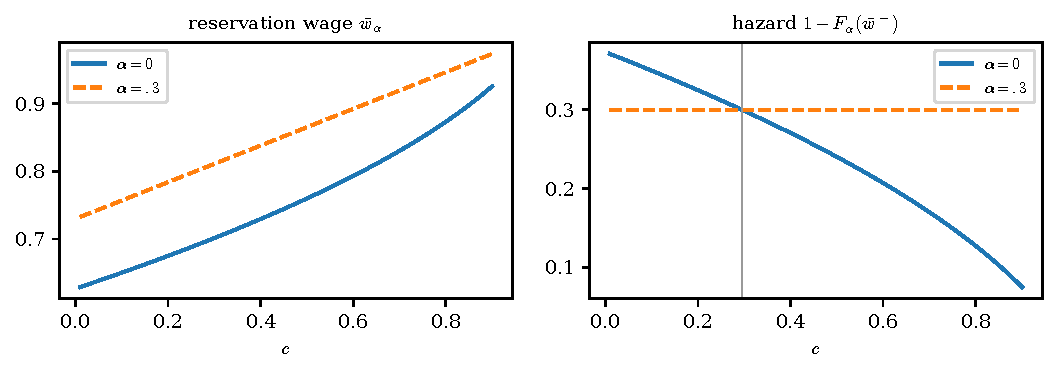
\includegraphics[width=0.95\linewidth]{fig/ls06_mps_atoms.pdf}\\[3pt]
\captionof{figure}{Exercise 6.20. Left: $\wb_{.3}>\wb_0$ for every $c$. Right: the exit hazards cross at $c^*=0.295$ (vertical line),
where $\wb_0=.7$ and type $.3$ starts to accept only the atom at $B$.}
\label{fig:atoms}
\end{center}
\end{tcolorbox}

%------- 6.21 -------
\begin{tcolorbox}[oddbox,title={Exercise 6.21 \quad Searching for the Lowest Price}]
\begin{tcolorbox}[questionbox]
(p.~218) At cost $c>0$ per draw a buyer draws a price offer $p\sim F$, $F(\underline B)=0$,
$F(\overline B)=1$; all search is within one period (no discounting); the buyer minimises price plus
search costs. (a) Optimal strategy. (b) Expected price net of all search costs.
\end{tcolorbox}

\textbf{Solution:}

\textbf{(a)} Let $V$ be the expected total outlay (price plus costs still to be paid) of a buyer about to pay
for a draw and behaving optimally. After drawing $p$ he either buys (pays $p$) or starts over (pays $V$
in expectation):
\[
V=c+\int\min\{p,V\}\,dF(p).
\]
So he buys iff $p\le\bar p\equiv V$: a \emph{reservation price}. Rearranging,
$c=\int[V-\min\{p,V\}]\,dF=\int_{\underline B}^{V}(V-p)\,dF(p)$, and integrating by parts,
\[
\boxed{c=\int_{\underline B}^{\bar p}F(p)\,dp}
\]
The right side is $0$ at $\bar p=\underline B$ and strictly increasing, so $\bar p$ is unique. If
$c\ge\int_{\underline B}^{\overline B}F=\overline B-Ep$, the equation has no root below $\overline B$: the buyer
takes the first draw and $\bar p=c+Ep$ (the formula $\int_{\underline B}^{\bar p}F=\bar p-Ep$ for $\bar p\ge\overline B$
gives the same number).

\textbf{(b)} The expected outlay is $V=\bar p$ itself. Decomposing: the number of draws is geometric with
success probability $F(\bar p)$, so expected costs are $c/F(\bar p)$, and the price paid has mean
$E[p\mid p\le\bar p]$; indeed $E[p\mid p\le\bar p]+c/F(\bar p)=\bar p$, because
$c=\int_{\underline B}^{\bar p}(\bar p-p)dF=F(\bar p)\{\bar p-E[p\mid p\le\bar p]\}$. (We read "purchase price net
of all search costs'' as price \emph{plus} search costs, the buyer's total outlay.)

\begin{tcolorbox}[databox]
$F$ uniform on $[1,2]$: $\bar p=1+\sqrt{2c}$ for $c\le\frac12$, $\bar p=c+1.5$ otherwise. $c=.02$: $1.2$ (simulated
outlay $1.1999$, $5.0$ draws); $c=.1$: $1.4472$ ($1.4482$); $c=.6$: $2.1$ (one draw). Minimising
$E[p\mid p\le x]+c/F(x)$ over $x$ gives the same $\bar p$.
\end{tcolorbox}
\end{tcolorbox}

%======================================================================
\subsection{Time-Varying Reservation Wages: Temporary Benefits and Seasons}
%======================================================================

%------- 6.14 -------
\begin{tcolorbox}[evenbox,title={Exercise 6.14 \quad Temporary Unemployment Compensation}]
\begin{tcolorbox}[questionbox]
(pp.~213--214) One offer per period, $F(0)=0$, $F(B)=1$; compensation $\gamma>0$ only in the \emph{first}
period of unemployment. (a) Bellman equations; the policy is a time-varying reservation wage. (b) How
does it vary with duration? (c) How does the hazard vary? Then compensation is also paid after a quit
(first period of a spell only; one period of work requalifies); an employed worker decides at the start
of a period whether to quit and, if so, draws an offer at once. (d) Bellman equations for $v^e(w)$,
$v^u_1(w')$, $v^u_+(w')$. (e) Characterise $\wb^e$, $\wb^u_1$, $\wb^u_+$ and relate them to $\gamma$.
\end{tcolorbox}

\textbf{Solution:}

\textbf{(a)} Let $v_1$ be the value in the first period of a spell (offer in hand, eligible for $\gamma$) and
$v_+$ afterwards:
\[
\boxed{v_1(w)=\max\Big\{\frac{w}{1-\beta},\,\gamma+\beta\int v_+\,dF\Big\},\qquad
v_+(w)=\max\Big\{\frac{w}{1-\beta},\,\beta\int v_+\,dF\Big\}}
\]
Both reject values are constants, so each period there is a reservation wage: $\wb_1=(1-\beta)(\gamma+\beta Ev_+)$
in the first period, $\wb_+=(1-\beta)\beta Ev_+$ afterwards.

\textbf{(b)} $v_+$ is McCall with $c=0$: $\wb_+=\frac{\beta}{1-\beta}\Gint{\wb_+}$. And
\[
\wb_1=\wb_++(1-\beta)\gamma .
\]
The reservation wage drops by $(1-\beta)\gamma$ after the first period and is constant thereafter.

\textbf{(c)} The hazard is $1-F(\wb_1)$ in the first period and $1-F(\wb_+)\ge1-F(\wb_1)$ from the second
period on: it rises (weakly) once, then stays flat.

\textbf{(d)} Accepting $w$ pays $w$ now and makes the worker "previously employed at $w$'' next period:
\[
\boxed{\begin{aligned}
v^e(w)&=\max\Big\{w+\beta v^e(w),\;\int v^u_1(w')\,dF(w')\Big\},\\
v^u_1(w')&=\max\Big\{w'+\beta v^e(w'),\;\gamma+\beta\int v^u_+\,dF\Big\},\\
v^u_+(w')&=\max\Big\{w'+\beta v^e(w'),\;\beta\int v^u_+\,dF\Big\}.
\end{aligned}}
\]
\textbf{(e)} Write $E_1=\int v^u_1dF$, $E_+=\int v^u_+dF$ and $A(w)=w+\beta v^e(w)$ (value of working at $w$ this
period).
\begin{enumerate}[label=\arabic*.,itemsep=3pt]
\item \emph{Quits.} By stationarity a worker either stays forever or quits now:
$v^e(w)=\max\{w/(1-\beta),E_1\}$, so $\boxed{\wb^e=(1-\beta)E_1}$, and
$A(w)=w/(1-\beta)$ for $w\ge\wb^e$, $A(w)=w+\beta E_1$ for $w<\wb^e$.
\item \emph{Ineligible unemployed.} $v^u_1\ge v^u_+$ pointwise ($\gamma>0$), so $E_1\ge E_+$. For every $w\ge0$,
$A(w)\ge w+\beta E_1\ge\beta E_+$: every offer is accepted, $\boxed{\wb^u_+=0}$. Taking any job requalifies the
worker, and he can quit next period with the benefit in hand.
\item \emph{Eligible unemployed.} $E_1\ge\gamma+\beta E_+$ (as $v^u_1\ge\gamma+\beta E_+$), so at $w=\wb^e$,
$A=E_1\ge\gamma+\beta E_+$: hence $\wb^u_1\le\wb^e$ and on that range $A=w+\beta E_1$, giving
$\wb^u_1=\gamma-\beta(E_1-E_+)$. Since all offers are accepted by the ineligible, $E_+=\int A\,dF$ and
$E_1-E_+=\int(\gamma+\beta E_+-A)^+dF=\int_0^{\wb^u_1}(\wb^u_1-w)\,dF=\int_0^{\wb^u_1}F(w)\,dw$. So
\[
\boxed{\wb^u_1+\beta\int_0^{\wb^u_1}F(w)\,dw=\gamma}
\]
The left side rises strictly from $0$, so $0<\wb^u_1\le\gamma$, increasing in $\gamma$; it depends only on
$\gamma$, $\beta$, $F$.
\item \emph{The parameter-dependent one.} Substituting $E_1=\wb^e/(1-\beta)$ in
$E_1=E_++\int_0^{\wb^u_1}F$ with $E_+=\int_{w<\wb^e}(w+\beta E_1)dF+\int_{w\ge\wb^e}\frac{w}{1-\beta}dF$, and using
$E\max\{w,x\}=Ew+\int_0^xF$:
\[
\boxed{\wb^e=Ew+\beta\int_0^{\wb^e}F(w)\,dw+(1-\beta)\int_0^{\wb^u_1}F(w)\,dw}
\]
So $\wb^e$ exceeds the mean wage and depends on the whole of $F$, on $\beta$, and on $\gamma$ only through the
small last term. Workers holding $w<\wb^e$ cycle: work one period, quit, collect $\gamma$ if the new draw is below
$\wb^u_1$, accept anything the next period, and so on.
\end{enumerate}

\begin{tcolorbox}[databox]
$F$ uniform on $[0,1]$, $\beta=.95$. (a)--(c): $\wb_+=.7239$ for all $\gamma$; $\wb_1=.7264,\ .7289,\ .7339$ for
$\gamma=.05,\ .1,\ .2$; hazards $.270$ then $.275$ at $\gamma=.1$ (simulated hazards by duration agree to
$4\times10^{-3}$). (d)--(e): $\wb^u_+=0$; $\wb^u_1=.0489,\ .0957,\ .1839$; $\wb^e=.8175,\ .8183,\ .8211$. VFI on the three
value functions reproduces all three cutoffs and the identity $E_1-E_+=\int_0^{\wb^u_1}F$.
\end{tcolorbox}
\end{tcolorbox}

%------- 6.15 -------
\begin{tcolorbox}[oddbox,title={Exercise 6.15 \quad Seasons, I}]
\begin{tcolorbox}[questionbox]
(p.~214) In odd periods the unemployed worker gets one offer from $F$, in even periods two; jobs last
forever. (a) Bellman equations. (b) Form of the optimal policy.
\end{tcolorbox}

\textbf{Solution:}

\textbf{(a)} Let $v_o(w)$, $v_e(w)$ be the values with best offer $w$ in hand in an odd (one-offer) and an even
(two-offer) period. Tomorrow is of the other type:
\[
\boxed{v_o(w)=\max\Big\{\frac{w}{1-\beta},\,c+\beta\int v_e\,dF^2\Big\},\qquad
v_e(w)=\max\Big\{\frac{w}{1-\beta},\,c+\beta\int v_o\,dF\Big\}}
\]
\textbf{(b)} Two reservation wages, $\wb_o=(1-\beta)Q_o$ and $\wb_e=(1-\beta)Q_e$, with
$Q_o=c+\beta\int\max\{\frac{w}{1-\beta},Q_e\}dF^2$, $Q_e=c+\beta\int\max\{\frac{w}{1-\beta},Q_o\}dF$.
\emph{Claim: $\wb_o>\wb_e$.} Suppose $Q_o\le Q_e$. Since $\varphi_Q(w)=\max\{w/(1-\beta),Q\}$ is nondecreasing in $w$ and
in $Q$, and $F^2$ first-order dominates $F$,
\[
Q_o=c+\beta\!\int\!\varphi_{Q_e}dF^2\ \ge\ c+\beta\!\int\!\varphi_{Q_o}dF^2\ \ge\ c+\beta\!\int\!\varphi_{Q_o}dF=Q_e ,
\]
so $Q_o=Q_e$ and both inequalities bind; but the second is strict whenever $(1-\beta)Q_o<B$ (then
$\int\varphi\,d(F^2-F)=\frac{1}{1-\beta}\int_{\wb}^BF(1-F)\,dw>0$). Contradiction, so $Q_o>Q_e$. The worker is
choosier in a one-offer period, because tomorrow brings two offers; the policy alternates between a high
and a low cutoff. Both lie between the stationary one-offer and two-offer reservation wages.

\begin{tcolorbox}[databox]
$F$ uniform on $[0,1]$, $c=.2$, $\beta=.95$: $\wb_o=.79794>\wb_e=.78744$; stationary benchmarks
$.75770$ (one offer always) and $.81434$ (two always). Two-equation root $=$ VFI on both functions.
\end{tcolorbox}
\end{tcolorbox}

%------- 6.16 -------
\begin{tcolorbox}[evenbox,title={Exercise 6.16 \quad Seasons, II}]
\begin{tcolorbox}[questionbox]
(pp.~214--215) One offer per period for the unemployed, no recall; the wage is fixed while in the job. At the
beginning of each odd period an employed worker is fired with probability $\pi\in(0,1)$ and immediately
draws a new offer; no firing in even periods. (a) Bellman equation. (b) Form of the optimal policy.
\end{tcolorbox}

\textbf{Solution:}

\textbf{(a)} Let $J_o(w)$, $J_e(w)$ be the values of working at $w$ during an odd/even period (after the firing
draw), and $v_o$, $v_e$ the values of an unemployed worker with offer $w$ in hand; $E_x=\int v_x\,dF$:
\[
\boxed{\begin{aligned}
J_o(w)&=w+\beta J_e(w), & J_e(w)&=w+\beta\big[(1-\pi)J_o(w)+\pi E_o\big],\\
v_o(w)&=\max\{J_o(w),\,c+\beta E_e\}, & v_e(w)&=\max\{J_e(w),\,c+\beta E_o\}.
\end{aligned}}
\]
(A fired worker immediately holds a fresh offer in an odd period, worth $E_o$ in expectation.)

\textbf{(b)} Solving the two linear equations, with $d\equiv1-\beta^2(1-\pi)$:
\[
J_e(w)=\frac{[1+\beta(1-\pi)]w+\beta\pi E_o}{d},\qquad J_o(w)=w+\beta J_e(w)=\frac{(1+\beta)w+\beta^2\pi E_o}{d},
\]
both strictly increasing, with slopes $s_e=\frac{1+\beta(1-\pi)}{d}$, $s_o=\frac{1+\beta}{d}$. The reject values are
constants, so the policy is \textbf{two reservation wages}: accept iff $w\ge\wb_o$ in odd periods and iff
$w\ge\wb_e$ in even periods, where $J_o(\wb_o)=c+\beta E_e$ and $J_e(\wb_e)=c+\beta E_o$.

\emph{Which is higher?} By the reduction of the overview, $E_o=c+\beta E_e+s_oG_o$ and $E_e=c+\beta E_o+s_eG_e$
with $G_x\equiv G_F(\wb_x)$. Hence $(1-\beta^2)E_o=(1+\beta)c+\beta s_eG_e+s_oG_o$.
\begin{itemize}[itemsep=2pt]
\item From $J_e(\wb_e)=c+\beta E_o$: $[1+\beta(1-\pi)]\wb_e=dc+\beta(d-\pi)E_o$, and $d-\pi=(1-\pi)(1-\beta^2)$. Substituting
$E_o$ and using $d+\beta(1-\pi)(1+\beta)=1+\beta(1-\pi)$:
\[
\wb_e=c+\frac{\beta(1-\pi)\,[\beta s_eG_e+s_oG_o]}{1+\beta(1-\pi)} .
\]
\item From $J_o(\wb_o)=c+\beta E_e=c(1+\beta)+\beta^2E_o+\beta s_eG_e$:
$(1+\beta)\wb_o=(1+\beta)dc+\beta^2(d-\pi)E_o+\beta\,d\,s_eG_e$; eliminating $E_o$ with the first bullet's
$\beta(d-\pi)E_o=[1+\beta(1-\pi)]\wb_e-dc$ and $ds_e=1+\beta(1-\pi)$:
\[
(1+\beta)\wb_o=dc+\beta[1+\beta(1-\pi)](\wb_e+G_e).
\]
\item Subtracting $(1+\beta)\wb_e$ and using $(1+\beta)-\beta[1+\beta(1-\pi)]=d$, then the first bullet for $c-\wb_e$
(with $d\,s_e=1+\beta(1-\pi)$, $d\,s_o=1+\beta$):
\[
\boxed{\wb_o-\wb_e=\frac{\beta}{1+\beta}\big[G_F(\wb_e)-\kappa\,G_F(\wb_o)\big],\qquad \kappa=\frac{(1-\pi)(1+\beta)}{1+\beta(1-\pi)}\in[0,1)}
\]
\end{itemize}
Fix $\wb_e$ and let $\psi(y)=y-\wb_e-\frac{\beta}{1+\beta}[G_F(\wb_e)-\kappa G_F(y)]$. Then
$\psi'(y)=1-\frac{\beta\kappa}{1+\beta}[1-F(y)]>0$, $\psi(\wb_o)=0$ and $\psi(\wb_e)=-\frac{\beta(1-\kappa)}{1+\beta}G_F(\wb_e)<0$ for
$\pi>0$, $\wb_e<B$. Hence $\boxed{\wb_o>\wb_e}$ (equal when $\pi=0$). Intuition: firing hands the worker a fresh
draw with no unemployment spell, which is valuable to someone holding a \emph{marginal} wage. A job
accepted in an even period faces its first firing draw after one period; one accepted in an odd period
locks the worker in for two. So the marginal wage is more attractive in even periods. For the same reason
both cutoffs fall as $\pi$ rises.

\begin{tcolorbox}[databox]
$F$ uniform on $[0,1]$, $\beta=.95$. $\pi=.3$, $c=.2$: $\wb_o=.57077$, $\wb_e=.56051$. Over
$\pi\in\{.1,.5,.9\}\times c\in\{0,.4,.8\}$ the gap ranges from $+.0002$ ($\pi=.1$, $c=.8$) to $+.178$ ($\pi=.9$, $c=0$),
and the boxed identity holds to $10^{-8}$. VFI on the four functions agrees with the closed form of $J$ plus a
two-equation root.
\end{tcolorbox}
\end{tcolorbox}

%======================================================================
\subsection{Quits, Promotions, Human Capital and Markov Wages}
%======================================================================

%------- 6.22 -------
\begin{tcolorbox}[evenbox,title={Exercise 6.22 \quad Quits}]
\begin{tcolorbox}[questionbox]
(pp.~218--219) One offer per period from $F$ for the unemployed. At the start of each period a worker
employed at $w$ has his job reclassified with probability $\alpha\in(0,1)$: he gets a new wage $w'\sim F$ and may
work at $w'$ until reclassified again, or quit (get $c$ now, draw next period). (a) Bellman equation for an
unemployed worker. (b) Decision rule of a previously unemployed worker. (c) Quit rule of a previously
employed worker. (d) How to compute the probability that a previously employed worker quits.
\end{tcolorbox}

\textbf{Solution:}

\textbf{(a)} Let $W(w)$ be the value of working at $w$ this period. Next period, with probability $\alpha$ the job is
reclassified and the worker is in exactly the position of an unemployed worker holding offer $w'$:
\[
\begin{gathered}\boxed{v(w)=\max\{W(w),\;c+\beta Ev\},\qquad W(w)=w+\beta\big[(1-\alpha)W(w)+\alpha Ev\big]}\\ Ev=\int v\,dF\end{gathered}
\]
so $W(w)=\dfrac{w+\beta\alpha Ev}{1-\beta(1-\alpha)}$, linear and increasing.

\textbf{(b)} Accept iff $W(w)\ge c+\beta Ev$, i.e.\ $w\ge\wb$. Let $D=1-\beta(1-\alpha)$ and $Q=c+\beta Ev$. Then
$Ev=Q+\frac{1}{D}G_F(\wb)$, so $(1-\beta)Ev=c+G_F(\wb)/D$. From $W(\wb)=Q$:
$\wb=DQ-\beta\alpha Ev=Dc+\beta(D-\alpha)Ev$ and $D-\alpha=(1-\alpha)(1-\beta)$, so
$\wb=Dc+\beta(1-\alpha)[c+G_F(\wb)/D]$, and with $D+\beta(1-\alpha)=1$:
\[
\boxed{\wb-c=\frac{\beta(1-\alpha)}{1-\beta(1-\alpha)}\int_{\wb}^B(w-\wb)\,dF(w)}
\]
McCall with the effective discount factor $\beta(1-\alpha)$: good jobs are less valuable because they may be
reclassified, so the worker is less choosy.

\textbf{(c)} A reclassified worker faces the same comparison $W(w')$ vs.\ $c+\beta Ev$: he keeps the new wage iff
$w'\ge\wb$ and quits otherwise. A worker who is not reclassified keeps $w\ge\wb$ (quitting would give
$Q\le W(w)$).

\textbf{(d)} Each period, $\Pr\{\text{quit}\mid\text{employed}\}=\alpha F(\wb)$, with $\wb$ from (b). The number of
periods until a quit is geometric with mean $1/[\alpha F(\wb)]$.

\begin{tcolorbox}[databox]
$F$ uniform on $[0,1]$, $c=.3$, $\beta=.95$, $\alpha=.2$: $\wb=.57970$, quit probability $\alpha F(\wb)=.11600$; a
simulation of 50\,000 workers for 200 periods, with decisions read off the VFI arrays, gives $.11607$.
\end{tcolorbox}
\end{tcolorbox}

%------- 6.23 -------
\begin{tcolorbox}[oddbox,title={Exercise 6.23 \quad A Career Ladder}]
\begin{tcolorbox}[questionbox]
(p.~219) One offer per period from $F$ for the unemployed. At the start of each period a worker employed
at $w$ is promoted with probability $\alpha$ to $\gamma w$, $\gamma>1$, until the next promotion. (a) Bellman equation for
a previously employed worker. (b) For a previously unemployed worker. (c) Decision rule of an unemployed
worker. (d) Decision rule of a previously employed worker.
\end{tcolorbox}

\textbf{Solution:}

\textbf{(a)} $\boxed{W(w)=w+\beta\big[(1-\alpha)W(w)+\alpha W(\gamma w)\big]}$. Guess $W(w)=kw$:
$k=1+\beta(1-\alpha)k+\beta\alpha\gamma k$, so
\[
W(w)=\frac{w}{\kappa},\qquad \kappa\equiv1-\beta(1-\alpha+\alpha\gamma),
\]
which requires $\beta(1-\alpha+\alpha\gamma)<1$ (otherwise the value is infinite). Check: $E[w_t]=w(1-\alpha+\alpha\gamma)^t$,
so $\sum_t\beta^tE[w_t]=w/\kappa$.

\textbf{(b)} $\boxed{v(w)=\max\{w/\kappa,\;c+\beta\int v\,dF\}}$.

\textbf{(c)} Accept iff $w\ge\wb$. With $Q=c+\beta Ev$ and $Ev=Q+G_F(\wb)/\kappa$, $\wb=\kappa Q$:
$\frac{\wb}{\kappa}=c+\frac{\beta\wb}{\kappa}+\frac{\beta G_F(\wb)}{\kappa}$, i.e.
\[
\boxed{(1-\beta)\wb=\kappa c+\beta\int_{\wb}^B(w-\wb)\,dF(w)}
\]
This is Exercise 6.8 with $\phi$ replaced by the expected growth factor $1-\alpha+\alpha\gamma$: promotions lower the
reservation wage when $c>0$ ($d\wb/d\gamma=-\beta\alpha c/[1-\beta F(\wb)]<0$).

\textbf{(d)} A previously employed worker stays and takes every promotion: wages only rise, so
$W(\gamma^jw)\ge W(w)\ge Q$ for $w\ge\wb$ and quitting (were it allowed) would never pay.

\begin{tcolorbox}[databox]
$F$ uniform on $[0,1]$, $c=.3$, $\beta=.95$, $\alpha=.1$, $\gamma=1.2$: $1/\kappa=32.258$ (Monte Carlo of promotion paths: $32.30$);
$\wb=.75522<.77613$ (no promotions). VFI agrees to $10^{-9}$.
\end{tcolorbox}
\end{tcolorbox}

%------- 6.24 -------
\begin{tcolorbox}[evenbox,title={Exercise 6.24 \quad Human Capital}]
\begin{tcolorbox}[questionbox]
(pp.~219--220) Offers pay $wh$, $w\sim F$; $w$ is kept during the job, $h$ follows a Markov chain $H^e$ when employed
(tends to rise) and $H^u$ when unemployed (tends to fall). At the start of a period employed workers
observe the new $h$ and may quit, keeping $h$ and drawing a new $w$ at once (accept it, or be unemployed at
least one period). (a) Bellman equation(s). (b) Describe the optimal rule; do employed workers ever quit?
(c) An algorithm.
\end{tcolorbox}

\textbf{Solution:}

\textbf{(a)} Let $S(w,h)$ be the value of working at $w$ this period with human capital $h$; $V^e(w,h)$ the value
of a worker employed last period at $w$ who has just observed $h$; $U(h)$ the value of an unemployed worker
about to draw $w$:
\[
\boxed{\begin{aligned}
S(w,h)&=wh+\beta\textstyle\sum_jH^e(h,j)\,V^e(w,\bar h_j),\qquad V^e(w,h)=\max\{S(w,h),\,U(h)\},\\
U(h)&=\displaystyle\int\max\Big\{S(w,h),\;c+\beta\textstyle\sum_jH^u(h,j)\,U(\bar h_j)\Big\}\,dF(w).
\end{aligned}}
\]
\textbf{(b)} By induction on the iterations, $S$ is nondecreasing in $w$, so both decisions are cutoffs:
\begin{itemize}[itemsep=2pt]
\item unemployed: accept iff $w\ge\wb^u(h)$, where $S(\wb^u(h),h)=R^u(h)\equiv c+\beta\sum_jH^u(h,j)U(\bar h_j)$;
\item employed: stay iff $w\ge\wb^e(h)$, where $S(\wb^e(h),h)=U(h)$.
\end{itemize}
Since $U(h)=\int\max\{S,R^u(h)\}dF\ge R^u(h)$, $\boxed{\wb^e(h)\ge\wb^u(h)}$, strictly when the draw has option value.
So employed workers \emph{do} quit: anyone whose $w$ lies below $\wb^e(h)$ at his current $h$ --- in particular
someone who accepted $w\in[\wb^u,\wb^e)$ quits as soon as next period. Accepting such a job is still
worthwhile: employment makes $h$ drift up (a rejecting worker's $h$ drifts down), it pays $wh$ now, and
quitting later gives an \emph{immediate} redraw, whereas rejecting costs a period of search. Quitting is
this model's form of on-the-job search. Rising $h$ also changes both cutoffs, so quits can follow human
capital shocks.

\textbf{(c)} (1) Grids for $w$ and the $n$ values $\bar h$. (2) Iterate the three equations as a map
$(V^e,U)\mapsto(V^e,U)$; it is a contraction with modulus $\beta$ (bounded payoffs, discounted
expectations), so it converges from any start. (3) Read off $\wb^u(h)$, $\wb^e(h)$. (4) Faster: Howard's
algorithm --- fix the cutoff rules, solve the linear system for $(S,U)$, improve, repeat.

\begin{tcolorbox}[databox]
$\bar h\in\{1,1.25,\dots,2\}$; $H^e$: up .4, stay .5, down .1; $H^u$: up .1, stay .5, down .4 (reflecting); $w$ uniform on $[0,1]$
(100 points), $c=.5$, $\beta=.95$. VFI (507 iterations) and Howard (6 improvements) give identical rules.
Acceptance cutoffs $\wb^u=(.165,.005,.005,.065,.185)$, quit cutoffs $\wb^e=(.845,.835,.825,.825,.815)$ across $h$:
the unemployed take almost any job and then quit into better draws. A simulated panel shows positive quits.
\end{tcolorbox}
\end{tcolorbox}

%------- 6.25 -------
\begin{tcolorbox}[oddbox,title={Exercise 6.25 \quad Markov Wages}]
\begin{tcolorbox}[questionbox]
(pp.~220--221) Successive offers follow a Markov chain on $\bar w_1<\dots<\bar w_n$ with transition matrix $P$; jobs are
permanent. (a) Bellman equation. (b) Can you prove the reservation-wage property? (c) With $\beta=.95$,
$c=1$, $\bar w=(1,\dots,5)$ and the given $P$, compute the optimal policy and value. (d) Same with $\beta=.99$.
(e) Discuss.
\end{tcolorbox}

\textbf{Solution:}

\textbf{(a)} $\boxed{v_i=\max\Big\{\dfrac{\bar w_i}{1-\beta},\;c+\beta\sum_jP_{ij}v_j\Big\}}$, $i=1,\dots,n$.

\textbf{(b)} Not in general. The reject value $c+\beta P_iv$ now depends on the current state because today's
offer predicts tomorrow's. The accept set is an upper set only if $\bar w_i/(1-\beta)-\beta P_iv$ is increasing in
$i$, which holds, e.g., for i.i.d.\ offers (identical rows) but can fail when a low wage forecasts high
future wages. The example has such a state: from $\bar w_3$ the chain jumps to $4$ or $5$ half the time.

\textbf{(c)--(d)} VFI, cross-checked by enumerating all $2^5=32$ accept/reject rules (each evaluated by solving
$v=r+\beta P_{\text{rej}}v$): the VFI value dominates all of them and is attained by the rule shown.
\begin{center}\small
\begin{tabular}{@{}lccccc@{}}
\toprule
state $i$ ($\bar w_i$) & 1 & 2 & 3 & 4 & 5\\
\midrule
$\beta=.95$: accept? & no & \textbf{yes} & no & no & yes\\
$\beta=.95$: $v_i$ & 35.833 & 40.000 & 61.834 & 80.312 & 100.000\\
$\beta=.99$: accept? & no & no & no & no & yes\\
$\beta=.99$: $v_i$ & 224.188 & 230.460 & 352.798 & 466.757 & 500.000\\
\bottomrule
\end{tabular}
\end{center}
\textbf{(e)} With $\beta=.95$ the policy is \emph{not} a reservation wage: $\bar w_2=2$ is accepted while $3$ and $4$ are
rejected. State 2 is persistent and mostly leads back to 1 or 2, so waiting there is expensive; state 3 is a
springboard (half the time next period's offer is 4 or 5), and state 4 is one step from 5 (probability
.18 per period). Check at state 2: rejecting is worth $1+.95(.18\cdot35.83+.8\cdot40+.02\cdot61.83)=38.70<40$. With
$\beta=.99$ the worker is patient enough to hold out for the top wage from every state: $5/(1-\beta)=500$
dwarfs the cost of a longer spell, and the policy becomes a (trivial) reservation wage $\bar w_5$. Higher patience
raises all values, weakly shrinks the accept set and restores monotonicity here.
\end{tcolorbox}

%======================================================================
\subsection{Search Intensity, Externalities and On-the-Job Investment}
%======================================================================

%------- 6.6 -------
\begin{tcolorbox}[evenbox,title={Exercise 6.6 \quad Mortensen Externality}]
\begin{tcolorbox}[questionbox]
(pp.~208--209) Worker and firm jointly draw a match $\theta\sim F$; matched pairs stay together forever, each
getting $\theta$ per period. Each side receives $n=f(c_1+c_2)$ offers per period, where $c_1$, $c_2$ are the
resources the worker and the typical firm devote to search, chosen at the start of the period; both have
the same reservation $\theta$. (a) Nash equilibrium: Bellman equations for $Q_i$, the value of an unmatched
type-$i$ agent before choosing $c_i$. (b) Planner maximising $\lambda\cdot$(utility 1) $+(1-\lambda)\cdot$(utility 2): Bellman
equation for $Q(\lambda)$. (c) Argue that Nash search is not optimal.
\end{tcolorbox}

\textbf{Solution:}

Timing: costs are paid, the $n$ draws arrive, the best one is accepted or not; an accepted match pays
$\theta$ from this period on, worth $\theta/(1-\beta)$; an unmatched agent gets nothing this period. Define
\[
M(n,R)\equiv\int\max\Big\{\frac{\theta}{1-\beta},R\Big\}\,dF^n(\theta)=R+\frac{1}{1-\beta}\int_{\bar\theta}^B\big[1-F(\theta)^n\big]\,d\theta,
\qquad\bar\theta=(1-\beta)R,
\]
the expected value of the best of $n$ draws when rejecting is worth $R$.

\textbf{(a)} Taking $c_j$ as given,
\[
\boxed{Q_i=\max_{c_i\ge0}\Big\{-c_i+\int\max\Big\{\frac{\theta}{1-\beta},\,\beta Q_i\Big\}\,dF^{f(c_i+c_j)}(\theta)\Big\}}
\]
that is, $Q_i=\max_{c_i}\{-c_i+M(f(c_i+c_j),\beta Q_i)\}$. Interior first-order condition: $1=f'(c_1+c_2)\,M_n\big(f(c_1+c_2),\beta Q_i\big)$, where
$M_n=-\frac{1}{1-\beta}\int_{\bar\theta}^BF^n\ln F\,d\theta>0$.

\textbf{(b)} Both parties receive the same $\theta$, so the weighted benefit is $\lambda\theta+(1-\lambda)\theta=\theta$, while the
weighted cost is $\lambda c_1+(1-\lambda)c_2$:
\[
\boxed{Q(\lambda)=\max_{c_1,c_2\ge0}\Big\{-\lambda c_1-(1-\lambda)c_2+\int\max\Big\{\frac{\theta}{1-\beta},\,\beta Q(\lambda)\Big\}\,dF^{f(c_1+c_2)}(\theta)\Big\}}
\]
Only $C=c_1+c_2$ matters for the benefit, so the planner loads search on the cheaper party and the
first-order condition is $\min\{\lambda,1-\lambda\}=f'(C)\,M_n(f(C),\beta Q(\lambda))$.

\textbf{(c)} In Nash, each party equates its \emph{private} marginal cost, $1$, to its private marginal benefit
$f'M_n$; but an extra unit of $c_i$ also raises the partner's chance of a good match by exactly the same
amount, an external benefit it ignores. The planner equates $f'M_n$ to $\min\{\lambda,1-\lambda\}\le\frac12<1$. With $f$
concave and $M_{nn}=-\frac{1}{1-\beta}\int F^n(\ln F)^2<0$, the product $f'(C)M_n(f(C),R)$ falls with $C$, so at a
given continuation value $R$ the planner chooses a larger $C$: \textbf{too few resources go to search in
the Nash equilibrium}. (The planner's higher $R$ lowers $M_n$ somewhat; the numerical example confirms
the ranking with $R$ endogenous.)

\begin{tcolorbox}[databox]
$\theta\sim U[0,1]$, $n=f(C)=1+4\sqrt C$ (real $n$, c.d.f.\ $\theta^n$), $\beta=.9$. Nash: $c_1=c_2=.1111$, $C=.2222$
($n=2.886$), $Q_i=8.0516$. Planner $\lambda=.5$: $C=.5495$ ($n=3.965$), value per agent $8.1412>8.0516$; $\lambda=.3$:
$C=.9453$. The closed form for $M$ matches quadrature; the Nash $c$ is a best response by direct
maximisation and satisfies the FOC.
\end{tcolorbox}
\end{tcolorbox}

%------- 6.11 -------
\begin{tcolorbox}[oddbox,title={Exercise 6.11 \quad Pissarides: Taxation and Variable Search Intensity}]
\begin{tcolorbox}[questionbox]
(p.~211) With effort $e$ the unemployed worker gets an offer $w\sim F$ with probability $\pi(e)$, $\pi(0)=0$,
$\pi'>0$, $\pi''<0$; a worker who accepts is fired with probability $\alpha$ per period. Flows: $1-e+z$ when searching
and not accepting; $w-e-T(w)$ in the first period of a job; $w-T(w)$ afterwards (taxes $T$, $w-T(w)$
increasing). (a) Show the policy is a reservation wage independent of $e$; display the condition for
$e$. (b) With $T(w)=t(w-a)$, show that a higher $a$ lowers the reservation wage and raises effort.
(c) When does a change in $t$ have the opposite effect?
\end{tcolorbox}

\textbf{Solution:}

\textbf{(a)} Let $n(w)=w-T(w)$, $D=1-\beta(1-\alpha)$. An employed worker's value (a fired worker is unemployed
next period, with value $U$ before choosing effort) is
\[
W(w)=n(w)+\beta[(1-\alpha)W(w)+\alpha U]\;\Longrightarrow\;W(w)=\frac{n(w)+\beta\alpha U}{D}.
\]
If the worker searches with effort $e$ and draws $w$: accept gives $W(w)-e$; reject gives $1-e+z+\beta U$.
\[
\boxed{\begin{aligned}U=\max_{e}\Big\{&(1-\pi(e))(1-e+z+\beta U)\\&+\pi(e)\int\max\{W(w)-e,\;1-e+z+\beta U\}\,dF(w)\Big\}\end{aligned}}
\]
The effort cost $e$ appears in both branches, so the accept/reject comparison is $W(w)$ vs.\ $1+z+\beta U$,
\emph{independent of $e$}; $W$ is increasing (as $n$ is), so accept iff $w\ge\wb$, $W(\wb)=1+z+\beta U$. Pulling
$1-e+z+\beta U$ out,
\[
U=1+z+\beta U+\max_e\big\{\pi(e)\Gamma(\wb)-e\big\},\qquad \Gamma(\wb)\equiv\int_{\wb}^B[W(w)-W(\wb)]\,dF,
\]
where $\Gamma(\wb)=\frac1D\int_{\wb}^B[n(w)-n(\wb)]\,dF$. So the effort condition is
\[
\boxed{\pi'(e)\,\Gamma(\wb)=1}\qquad\text{(interior)}.
\]
\emph{The reservation equation.} From $W(\wb)=1+z+\beta U$: $n(\wb)=D(1+z)+\beta(D-\alpha)U$, with $D-\alpha=(1-\alpha)(1-\beta)$ and
$(1-\beta)U=1+z+\pi(e)\Gamma-e$. Since $D+\beta(1-\alpha)=1$,
\[
n(\wb)=1+z+\beta(1-\alpha)\max_e\{\pi(e)\Gamma(\wb)-e\}.
\]
\textbf{(b)} With $T=t(w-a)$: $n(w)=(1-t)w+ta$, $\Gamma=(1-t)G_F(\wb)/D$. Define
\[
\begin{gathered}\Phi(\wb;a,t)=(1-t)\wb+ta-1-z-\beta(1-\alpha)\,\mathcal M(\wb,t),\\ \mathcal M=\max_e\Big\{\pi(e)\frac{(1-t)G_F(\wb)}{D}-e\Big\}.\end{gathered}
\]
By the envelope theorem $\mathcal M_{\wb}=-\pi(e)(1-t)[1-F(\wb)]/D$, so
$\Phi_{\wb}=(1-t)\big[1+\beta(1-\alpha)\pi(e)(1-F(\wb))/D\big]>0$, and $\Phi_a=t>0$. Hence
\[
\frac{d\wb}{da}=-\frac{t}{\Phi_{\wb}}<0 .
\]
Effort solves $\pi'(e)=D/[(1-t)G_F(\wb)]$; $\wb\downarrow\Rightarrow G_F(\wb)\uparrow\Rightarrow\pi'(e)\downarrow\Rightarrow e\uparrow$ ($\pi''<0$). Both raise
the acceptance probability $\pi(e)[1-F(\wb)]$. A larger exemption raises the net income of every job by $ta$
without touching the unemployed.

\textbf{(c)} $\mathcal M_t=-\pi(e)G_F(\wb)/D$, so $\Phi_t=a-\wb+\beta(1-\alpha)\pi(e)G_F(\wb)/D$. Using the reservation equation,
$\beta(1-\alpha)\pi(e)G_F/D=[(1-t)\wb+ta-1-z+\beta(1-\alpha)e]/(1-t)$, which gives
\[
\Phi_t=\frac{a-(1+z)+\beta(1-\alpha)e}{1-t},\qquad
\frac{d\wb}{dt}=-\frac{\Phi_t}{\Phi_{\wb}}>0\iff \boxed{a<1+z-\beta(1-\alpha)e}.
\]
Under that condition a higher $t$ raises $\wb$; and effort falls, since $\pi'(e)=D/[(1-t)G_F(\wb)]$ rises both
because $1-t$ falls and because $G_F(\wb)$ falls. That is the opposite of an increase in $a$. When the
exemption is large, $a>1+z-\beta(1-\alpha)e$, the tax is a net subsidy at the margin (it is negative for
$w<a$), and $\wb$ falls with $t$; the effect on effort is then ambiguous.

\begin{tcolorbox}[databox]
$\pi(e)=1-e^{-2e}$, $F$ uniform on $[0,5]$, $\beta=.95$, $\alpha=.1$, $z=.5$. At $a=1$, $t=.3$: $\wb=2.8723$, $e=.7375$ (literal VFI on
$w$ and $e$ grids: $2.8725$, $.7375$); $d\wb/da=-.146$, $de/da=+.069$. At $a=.2$: threshold $.919>a$,
$d\wb/dt=+.532$, $de/dt=-.979$. At $a=2.5$: threshold $.790<a$, $d\wb/dt=-1.080$, $de/dt=-.252$. The analytic
$d\wb/dt$ matches the finite difference to $10^{-5}$.
\end{tcolorbox}
\begin{center}
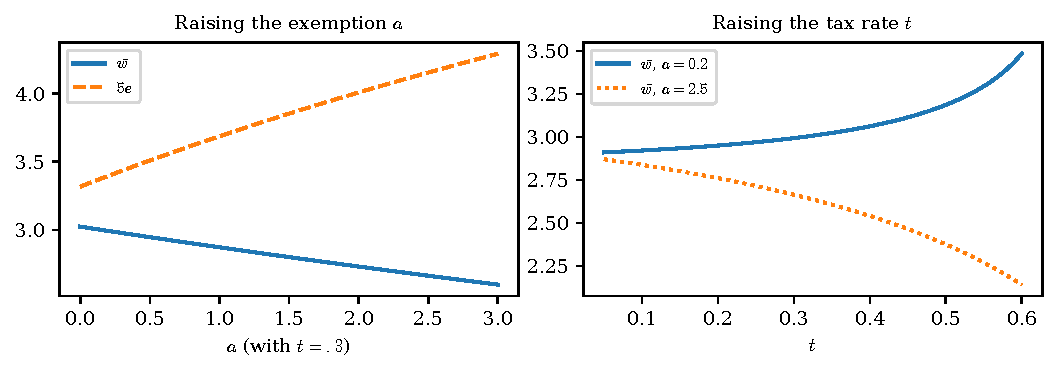
\includegraphics[width=0.95\linewidth]{fig/ls06_pissarides.pdf}\\[3pt]
\captionof{figure}{Exercise 6.11. Left: raising the exemption $a$ lowers $\wb$ and raises effort. Right: raising $t$
raises $\wb$ when $a=.2$ (below the threshold) and lowers it when $a=2.5$.}
\label{fig:piss}
\end{center}
\end{tcolorbox}

%------- 6.18 -------
\begin{tcolorbox}[evenbox,title={Exercise 6.18 \quad Jovanovic (1979b)}]
\begin{tcolorbox}[questionbox]
(p.~216) An employed worker earns $w_t=x_t(1-\phi_t-s_t)$: $x_t$ job-specific capital, $\phi_t$ time invested in it, $s_t$
time searching. Searching $s_t$ brings, with probability $\pi(s_t)$, an offer to restart at capital $\mu'\sim F$ next
period ($\pi'>0$, $\pi''<0$). On the job $x_{t+1}=G(x_t,\phi_t)$, printed as $g(x_t\phi_t)-\delta x_t$; $x_0=\mu$. Risk
neutral, discount $\beta$. (a) Bellman equation. (b) Rule for accepting $\mu'$. (c) With $g(x\phi)=A(x\phi)^\alpha$,
$\pi(s)=s^{.5}$, $F$ discrete on $n$ values, compute and display the optimal $\phi$, $s$.
\end{tcolorbox}

\textbf{Solution:}

\emph{Misprint.} As printed, $x_{t+1}=g(x_t\phi_t)-\delta x_t$ is negative whenever $\phi_t$ is small (e.g.\ $\phi_t=0$
gives $-\delta x_t$), which is impossible for a capital stock and inconsistent with calling $\delta$ a depreciation
rate. We use
\[
x_{t+1}=G(x_t,\phi_t)=(1-\delta)x_t+g(x_t\phi_t).
\]
\textbf{(a)} Let $x'=G(x,\phi)$:
\[
\boxed{\begin{aligned}V(x)=\max_{\phi,s\ge0,\ \phi+s<1}\Big\{&x(1-\phi-s)\\&+\beta\Big[(1-\pi(s))V(x')+\pi(s)\int\max\{V(x'),V(\mu')\}\,dF(\mu')\Big]\Big\}\end{aligned}}
\]
\textbf{(b)} $V$ is increasing: more capital raises this period's earnings for any $(\phi,s)$ and, since
$G_x=(1-\delta)+\phi g'>0$, next period's capital. So the worker accepts $\mu'$ iff $V(\mu')>V(x')$, i.e.\ iff
$\boxed{\mu'>x_{t+1}}$: the reservation match is the capital he would carry on the current job.
(Under the printed law $G_x=\phi g'-\delta$ can be negative and this monotonicity argument breaks.)

\emph{First-order conditions.} Let $K(x')=\int\max\{V(\mu')-V(x'),0\}dF$ (option value of an offer). The
objective is $x(1-\phi-s)+\beta[V(x')+\pi(s)K(x')]$:
\[
s:\ x=\beta\pi'(s)K(x'),\qquad
\phi:\ 1=\beta g'(x\phi)\,V'(x')\,\big[1-\pi(s)(1-F(x'))\big].
\]
Search trades current earnings for the option $K$; investment pays only if the worker stays, which
happens with probability $1-\pi(s)[1-F(x')]$. With $\pi(s)=\sqrt s$ the first condition gives
$s=\big(\beta K(x')/2x\big)^2$ (capped by the time constraint), so only $\phi$ needs a grid search.

\textbf{(c)} Parameters (not given in the book): $A=1$, $\alpha=.5$, $\delta=.1$, $\beta=.95$, $\mu\in\{5,10,\dots,45\}$ with $f_i=1/9$,
$x\in[.5,100]$ (300 points, linear interpolation), $\phi$ on 400 points, $s\le.999-\phi$ so that $\pi(s)<1$.

\begin{tcolorbox}[databox]
VFI converges in 468 iterations. $V$ is strictly increasing. For $x\le12.15$ the worker spends all his time
searching ($\phi=0$, $s=.999$); search then falls fast ($s(20)=.32$) and stops once $x$ exceeds every
possible $\mu$ ($s(45)\approx0$); investment is hump-shaped ($\phi(20)=.003$, $\phi(45)=.129$, $\phi(80)=.120$). A
brute-force $(\phi,s)$ grid at $x=3,20,60$ reproduces $V$ within $0.2\%$; Monte Carlo of the policy
(2\,000 paths, 200 periods) gives $491.2\pm1.2$ vs.\ $V(5)=489.5$ and $514.4\pm1.1$ vs.\ $V(30)=513.8$.
\end{tcolorbox}
\begin{center}
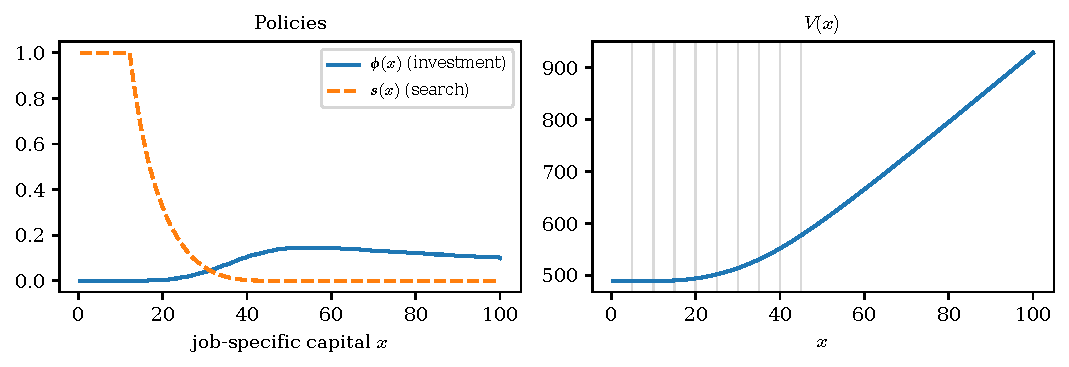
\includegraphics[width=0.95\linewidth]{fig/ls06_jovanovic.pdf}\\[3pt]
\captionof{figure}{Exercise 6.18. Left: investment $\phi(x)$ and search $s(x)$. Right: $V(x)$; grey lines mark the possible
new matches $\mu$.}
\label{fig:jov}
\end{center}
\end{tcolorbox}

%======================================================================
\subsection{Computation: Value Iteration, Policy Improvement and Gittins Indexes}
%======================================================================

%------- 6.19 -------
\begin{tcolorbox}[oddbox,title={Exercise 6.19 \quad Value Function Iteration and Policy Improvement}]
\begin{tcolorbox}[questionbox]
(p.~217) McCall's model. (a) Bellman equation; reservation-wage policy; equation for $w^*$. (b) VFI: show the
policy at each iteration is a reservation wage $w_n$; derive a recursion; show $w_n\to w^*$ at rate $\beta$.
(c) Howard's algorithm: same, and show local quadratic convergence, $w_{n+1}-w^*\cong K(w_n-w^*)^2$.
\end{tcolorbox}

\textbf{Solution:}

\textbf{(a)} $v(w)=\max\{w/(1-\beta),\,c+\beta\int v\,dF\}$; accept iff $w\ge w^*$ with
$w^*-c=\frac{\beta}{1-\beta}\int_{w^*}^B(w-w^*)dF$, equivalently $w^*=(1-\beta)c+\beta\int\max\{w,w^*\}dF$.

\textbf{(b)} Start from $v_0\equiv0$. Then $v_1(w)=\max\{w/(1-\beta),c\}$, a cutoff at $w_1=(1-\beta)c$. If
$v_n(w)=\max\{w,w_n\}/(1-\beta)$, then $v_{n+1}(w)=\max\{w/(1-\beta),\,c+\beta Ev_n\}$ is again a cutoff rule (accept value
increasing, reject value constant) with
\[
\boxed{w_{n+1}=T(w_n)\equiv(1-\beta)c+\beta\int\max\{w,w_n\}\,dF(w)=(1-\beta)c+\beta\big[w_n+G_F(w_n)\big]}
\]
$T'(x)=\beta[1+G_F'(x)]=\beta F(x)\in[0,\beta]$, so by the mean value theorem
$|w_{n+1}-w^*|=|T(w_n)-T(w^*)|\le\beta|w_n-w^*|$: linear convergence at rate at most $\beta$; asymptotically the
rate is exactly $\beta F(w^*)$.

\textbf{(c)} \emph{Evaluation.} The rule "accept iff $w\ge w_n$'' is worth $w/(1-\beta)$ for $w\ge w_n$ and $Q_n$
otherwise, with $Q_n=c+\beta\big[F(w_n)Q_n+\frac{1}{1-\beta}\int_{w_n}^Bw\,dF\big]$, so
$Q_n=\dfrac{c+\frac{\beta}{1-\beta}\int_{w_n}^Bw\,dF}{1-\beta F(w_n)}$.
\emph{Improvement.} Maximise $\max\{w/(1-\beta),\,c+\beta Ev_{\text{pol}}\}$; the constant is $c+\beta Ev_{\text{pol}}=Q_n$, so the new
policy is again a cutoff:
\[
\boxed{w_{n+1}=H(w_n)\equiv\frac{(1-\beta)c+\beta\int_{w_n}^Bw\,dF(w)}{1-\beta F(w_n)}}
\]
\emph{Fixed point.} $H(w^*)=w^*\iff w^*(1-\beta F(w^*))=(1-\beta)c+\beta\int_{w^*}w\,dF\iff w^*=(1-\beta)c+\beta\int\max\{w,w^*\}dF$,
the equation of (a).
\emph{Derivative} (quotient rule, $\frac{d}{dx}\int_x^Bw\,dF=-xf(x)$):
\[
H'(x)=\frac{-\beta xf(x)[1-\beta F(x)]+\beta f(x)\big[(1-\beta)c+\beta\int_x^Bw\,dF\big]}{[1-\beta F(x)]^2}=\frac{\beta f(x)\,[H(x)-x]}{1-\beta F(x)},
\]
so $H'(w^*)=0$, and differentiating once more at $w^*$ (the term multiplying $H-x$ drops out):
$H''(w^*)=\frac{\beta f(w^*)[H'(w^*)-1]}{1-\beta F(w^*)}=-\frac{\beta f(w^*)}{1-\beta F(w^*)}$. A second-order Taylor expansion gives
\[
w_{n+1}-w^*=H(w_n)-H(w^*)\cong\tfrac12H''(w^*)(w_n-w^*)^2,\qquad
\boxed{K=-\frac{\beta f(w^*)}{2[1-\beta F(w^*)]}}
\]
$K<0$: after the first step Howard approaches $w^*$ from below, doubling the number of correct digits each
step. It is Newton's method on $w-T(w)=0$: indeed $H(x)=x-\frac{x-T(x)}{1-T'(x)}$.

\begin{tcolorbox}[databox]
$F$ uniform on $[0,1]$, $c=.3$, $\beta=.95$: $w^*=0.7761278834$. VFI ratio $(w_{n+1}-w^*)/(w_n-w^*)\to0.737321=\beta F(w^*)$
(every ratio $<\beta$). Howard from $w_0=0$: $0.49,\ 0.703372,\ 0.768550,\ 0.776027,\ 0.776128$; measured
$(w_{n+1}-w^*)/(w_n-w^*)^2=-1.760,\ -1.808$ vs.\ $K=-1.8083$. Both scalar recursions are reproduced by
whole-function VFI and policy evaluation on a 4000-point grid.
\end{tcolorbox}
\begin{center}
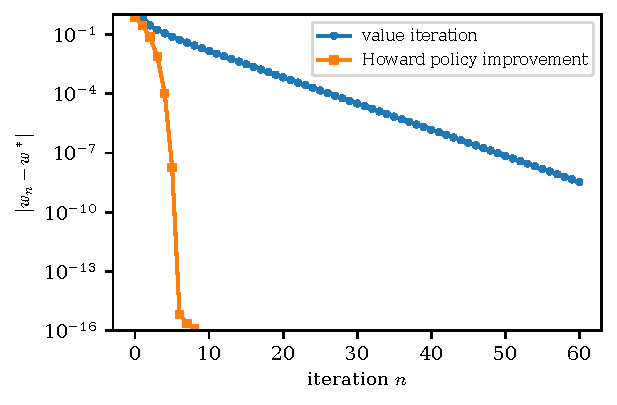
\includegraphics[width=0.6\linewidth]{fig/ls06_howard.pdf}\\[3pt]
\captionof{figure}{Exercise 6.19. Error $|w_n-w^*|$: linear for value iteration (rate $\beta F(w^*)=.737$), quadratic for Howard (machine
precision after six steps).}
\label{fig:howard}
\end{center}
\end{tcolorbox}

%------- 6.17 -------
\begin{tcolorbox}[oddbox,title={Exercise 6.17 \quad Gittins Indexes for Beginners}]
\begin{tcolorbox}[questionbox]
(pp.~215--216) Two jobs, A and B, with wages driven by job-specific $n$-state Markov chains $A=[A_{ij}]$, $B=[B_{IJ}]$ and
wages $w_a(i)$, $w_b(I)$. At the end of each period the worker chooses the job for next period, before seeing
next period's wage; a job he returns to restarts from his last state there. No unemployment.
(a) Bellman equation for a worker whose last states were $i$ on A and $I$ on B. (b) For a new worker whose
first wage on A (B) is drawn from $\pi_a$ ($\pi_b$).
\end{tcolorbox}

\textbf{Solution:}

\textbf{(a)} Let $V(i,I)$ be the value at the end of a period with last states $i$ and $I$. Working at A next period
moves A's state to $j$ with probability $A_{ij}$, pays $w_a(j)$, and leaves B's state frozen at $I$:
\[
\boxed{V(i,I)=\max\Big\{\sum_jA_{ij}\big[w_a(j)+\beta V(j,I)\big],\;\sum_JB_{IJ}\big[w_b(J)+\beta V(i,J)\big]\Big\}}
\]
\textbf{(b)} Following the hint, $v_a(i)$ is the value of a worker last in state $i$ on A who has never worked on B (B
would start from $\pi_b$); $v_b(I)$ symmetrically:
\[
\boxed{\begin{aligned}
v_a(i)&=\max\Big\{\sum_jA_{ij}[w_a(j)+\beta v_a(j)],\;\sum_J\pi_{bJ}[w_b(J)+\beta V(i,J)]\Big\},\\
v_b(I)&=\max\Big\{\sum_JB_{IJ}[w_b(J)+\beta v_b(J)],\;\sum_i\pi_{ai}[w_a(i)+\beta V(i,I)]\Big\},\\
\text{new worker: }&\max\Big\{\sum_i\pi_{ai}[w_a(i)+\beta v_a(i)],\;\sum_I\pi_{bI}[w_b(I)+\beta v_b(I)]\Big\}.
\end{aligned}}
\]
Equivalently, add a "fresh'' state $0$ to each chain with transition row $\pi_a$ (resp.\ $\pi_b$): then
$v_a(i)=V(i,0_b)$, $v_b(I)=V(0_a,I)$ and the new worker's value is $V(0_a,0_b)$.

\emph{Why "Gittins''.} This is a two-armed bandit: the idle job's state is frozen. By the Gittins index
theorem the optimal rule is to work at the job whose current state has the larger index
$\nu(k)=(1-\beta)M_k(k)$, where $M_k$ solves the one-job "restart in $k$'' problem
$M_k(i)=\max\{r(i)+\beta\sum_jP_{ij}M_k(j),\;r(k)+\beta\sum_jP_{kj}M_k(j)\}$, $r(i)=\sum_jP_{ij}w(j)$. The two-dimensional
Bellman equation collapses to two one-dimensional indexes.

\begin{tcolorbox}[databox]
$n=4$, random (seeded) $A$, $B$, wages on $[0,10]$, $\pi_a$, $\pi_b$; $\beta=.9$. Indexes: A $(5.858,5.985,6.075,5.278)$,
B $(6.289,5.926,4.899,4.595)$. At every $(i,I)$ where they differ, the choice from $V$ equals the choice of the
larger index. The hint equations and the augmented-chain formulation agree; a new worker starts at B
(value $55.780$ vs.\ $55.705$; fresh-state indexes $6.264$ vs.\ $5.852$).
\end{tcolorbox}
\end{tcolorbox}

%======================================================================
\subsection{Neal's Model of Career Choice}
%======================================================================

%------- 6.26 -------
\begin{tcolorbox}[evenbox,title={Exercise 6.26 \quad Neal Model's Markov Implications}]
\begin{tcolorbox}[questionbox]
(pp.~221--222) Partition the $(\theta,\epsilon)$ space of Neal's model with Figure 6.5.2 into $s=1$ (wants a new life), $s=2$
(keeps career, wants a new job), $s=3$ (stays put); $P_{ij}=\Pr(s_{t+1}=j\mid s_t=i)$, $\Pr(s_0=1)=1$. (a) Show
$P=\begin{bmatrix}1-P_{12}-P_{13}&P_{12}&P_{13}\\0&1-P_{23}&P_{23}\\0&0&1\end{bmatrix}$ and say how to compute its elements. (b)
Invariant distribution(s). (c) Is the chain ergodic? (d) How could quarterly panel data on job and
occupation switches be used to estimate $P$?
\end{tcolorbox}

\textbf{Solution:}

\emph{Facts from section 6.5.} $Q=\iint[\theta'+\epsilon'+\beta v]dFdG$, $C(\theta)=\theta+\int[\epsilon'+\beta v(\theta,\epsilon')]dG$,
$C(\bar\theta)=Q$ (6.5.4). For $\theta\ge\bar\theta$ the career is kept forever and the job cutoff $\bar\epsilon$ solves the
McCall equation (6.5.5), \emph{independent of $\theta$}. For $\theta<\bar\theta$ the worker stays iff $\theta+\epsilon\ge(1-\beta)Q$ and
otherwise takes a new life. So: region 3 $=\{\theta\ge\bar\theta,\epsilon\ge\bar\epsilon\}\cup\{\theta<\bar\theta,\theta+\epsilon\ge(1-\beta)Q\}$,
region 2 $=\{\theta\ge\bar\theta,\epsilon<\bar\epsilon\}$, region 1 the rest.

\textbf{(a)} \emph{Row 3.} A worker who stays put keeps $(\theta,\epsilon)$ and stays put again: $P_{33}=1$.
\emph{Row 2.} Here $\theta\ge\bar\theta$, the career is kept and only $\epsilon'\sim G$ is new; the new pair has
$\theta\ge\bar\theta$, so it is never in region 1 ($P_{21}=0$), and it is in region 3 iff $\epsilon'\ge\bar\epsilon$, whatever $\theta$:
\[
P_{23}=1-G(\bar\epsilon^-),\qquad P_{22}=G(\bar\epsilon^-).
\]
Because $\bar\epsilon$ does not depend on $\theta$, row 2 is the same for every $\theta$ in region 2, which is what makes
$s$ a Markov state. \emph{Row 1.} A fresh pair $(\theta',\epsilon')\sim F\times G$:
\[
\begin{gathered}P_{12}=[1-F(\bar\theta^-)]\,G(\bar\epsilon^-),\qquad P_{13}=\iint\mathbf 1\{(\theta',\epsilon')\in\text{region 3}\}\,dF\,dG,\\ P_{11}=1-P_{12}-P_{13}.\end{gathered}
\]
\emph{Computation.} Solve (6.5.1) by VFI on the grid used for Figure 6.5.2; read off $Q$, $C(\theta)$, $\bar\theta$,
$\bar\epsilon$; sum the grid probabilities of each region.

\textbf{(b)} $\pi'P=\pi'$: column 1 gives $\pi_1(1-P_{12}-P_{13})=\pi_1\Rightarrow\pi_1=0$ (as $P_{12}+P_{13}>0$); column 2 gives
$\pi_1P_{12}+\pi_2(1-P_{23})=\pi_2\Rightarrow\pi_2P_{23}=0\Rightarrow\pi_2=0$. The unique invariant distribution is
$\boxed{\pi_\infty=(0,0,1)}$, and from $\pi_0=(1,0,0)$, $\pi_t\to\pi_\infty$: everyone eventually settles in a job and career.

\textbf{(c)} States 1 and 2 are transient and 3 is absorbing, so the chain is not irreducible. But it has a unique
stationary distribution, and every invariant function is (trivially) constant on its support $\{3\}$: in the
sense of section 2.2.7 the chain \emph{is} ergodic, and time averages of any $y(s_t)$ converge to $y(3)$ from any
initial state, since absorption occurs with probability one.

\textbf{(d)} The state is revealed by the next move. For each worker and quarter $t$: a switch of job
\emph{and} occupation at $t+1$ means $s_t=1$; a switch of job only means $s_t=2$; no switch means $s_t=3$.
This gives each worker's sequence $s_0=1,s_1,\dots$ (the last quarter is censored). The maximum-likelihood
estimator of a Markov chain is the matrix of transition frequencies, with the model's zeros imposed:
\[
\hat P_{12}=\frac{n_{12}}{n_{1\cdot}},\quad\hat P_{13}=\frac{n_{13}}{n_{1\cdot}},\quad\hat P_{23}=\frac{n_{23}}{n_{2\cdot}},\qquad
\text{s.e.}(\hat P_{ij})=\sqrt{\hat P_{ij}(1-\hat P_{ij})/n_{i\cdot}},
\]
$n_{ij}$ the number of $i\to j$ transitions. Practical issues: a model period need not be a quarter (several
switches in a quarter, or quarters without a decision); the model's prediction that a worker who has not
switched never switches again (and never leaves region 2 for region 1) is testable, and violations point
to learning (Jovanovic, section 6.8) or heterogeneity; with $P$ in hand one can go further and pick $F$, $G$,
$\beta$ to match $\hat P$ (minimum distance).

\begin{tcolorbox}[databox]
Neal's parameters (50-point uniform grids on $[0,5]$, $\beta=.95$): $\bar\theta=3.980$, $\bar\epsilon=4.184$ (as in Figure 6.5.2),
\[
P=\begin{bmatrix}.7620&.1804&.0576\\0&.8200&.1800\\0&0&1\end{bmatrix}.
\]
Row 2 is identical for all 11 careers in region 2. A simulated panel of 5\,000 workers over 40 periods,
treated as in (d), gives $\hat P_{12}=.1813$, $\hat P_{13}=.0576$, $\hat P_{23}=.1782$, all within 4 standard errors.
\end{tcolorbox}
\end{tcolorbox}

%------- 6.27 -------
\begin{tcolorbox}[oddbox,title={Exercise 6.27 \quad Neal Model with Unemployment}]
\begin{tcolorbox}[questionbox]
(p.~222) As in Neal's model, but a worker who wants a new job, or a new career and job, must be unemployed
this period (receiving $c$) and draws $\epsilon'$ (or $(\theta',\epsilon')$) for next period. (a) Bellman equation for
$v(\theta,\epsilon)$. (b) Characterise the optimal policy.
\end{tcolorbox}

\textbf{Solution:}

\textbf{(a)}
\[
\boxed{\begin{aligned}v(\theta,\epsilon)=\max\Big\{&\theta+\epsilon+\beta v(\theta,\epsilon),\;\;c+\beta\int v(\theta,\epsilon')\,dG(\epsilon'),\\&c+\beta\iint v(\theta',\epsilon')\,dF(\theta')\,dG(\epsilon')\Big\}\end{aligned}}
\]
\textbf{(b)} Staying put, once optimal, is optimal forever and is worth $(\theta+\epsilon)/(1-\beta)$. Let
$C(\theta)=c+\beta\int v(\theta,\epsilon')dG$ and $Q=c+\beta\iint v\,dFdG$. $v$ is nondecreasing in $\theta$ (by induction on
VFI), so $C$ is nondecreasing and there is a cutoff $\bar\theta$ with $C(\theta)\ge Q$ iff $\theta\ge\bar\theta$.
\begin{itemize}[itemsep=2pt]
\item $\theta<\bar\theta$: a new job is dominated by a new life. Stay iff $\theta+\epsilon\ge(1-\beta)Q$ (a diagonal boundary), otherwise
new life.
\item $\theta\ge\bar\theta$: the career is never abandoned (a new job leaves $\theta$ unchanged). The problem is McCall with
offers $\theta+\epsilon'$ and compensation $c$: $v(\theta,\epsilon)=\max\{\frac{\theta+\epsilon}{1-\beta},\,c+\beta\int v(\theta,\epsilon')dG\}$. Stay iff
$\epsilon\ge\bar\epsilon(\theta)$ with
\[
\theta+\bar\epsilon(\theta)-c=\frac{\beta}{1-\beta}\int_{\bar\epsilon(\theta)}(\epsilon'-\bar\epsilon(\theta))\,dG(\epsilon'),
\qquad
\frac{d\bar\epsilon}{d\theta}=-\frac{1}{1+\frac{\beta}{1-\beta}[1-G(\bar\epsilon)]}\in(-1,0).
\]
\end{itemize}
\emph{Contrast with Neal.} There $\bar\epsilon$ is independent of $\theta$ because a new job is drawn at once and the
career income $\theta$ is earned regardless. Here looking for a new job costs a period of career income
($\theta$ replaced by $c$), so workers in better careers are less choosy about jobs: $\bar\epsilon(\theta)$ slopes down, while
$\theta+\bar\epsilon(\theta)$ still rises. The three regions keep the shape of Figure 6.5.2, but the new-job/stay boundary
now slopes down.

\begin{tcolorbox}[databox]
Same grids, $\beta=.95$, $c=1$: $\bar\theta=3.673$ (vs.\ $3.980$ without unemployment); $\bar\epsilon(\theta)$ falls from $3.265$ at
$\theta=3.673$ to $3.098$ at $\theta=5$. For every $\theta\ge\bar\theta$ the VFI stay region coincides with $\epsilon\ge\bar\epsilon(\theta)$ from the McCall
equation, and for $\theta<\bar\theta$ with $\theta+\epsilon\ge(1-\beta)Q$.
\end{tcolorbox}
\begin{center}
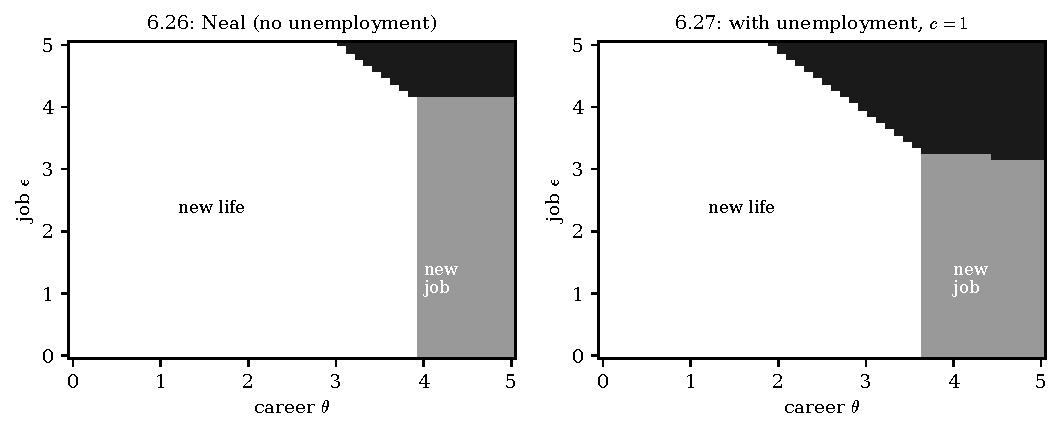
\includegraphics[width=0.95\linewidth]{fig/ls06_neal.pdf}\\[3pt]
\captionof{figure}{Exercises 6.26--6.27. Decision regions: white $=$ new life, grey $=$ new job, black $=$ stay put.
Left: Neal's model (reproduces Figure 6.5.2). Right: with unemployment while searching, $c=1$.}
\label{fig:neal}
\end{center}
\end{tcolorbox}

%======================================================================
\section*{Book misprints and caveats}
\addcontentsline{toc}{section}{Book misprints and caveats}
%======================================================================
\begin{itemize}[itemsep=3pt]
\item \textbf{Exercise 6.18, law of motion.} Printed $x_{t+1}=g(x_t\phi_t)-\delta x_t$ gives negative capital for small
$\phi_t$; read as $x_{t+1}=(1-\delta)x_t+g(x_t\phi_t)$.
\item \textbf{Exercise 6.8.} "The economy with the higher growth rate has the smaller reservation wage'' holds
strictly only for $c>0$; with $c=0$ the reservation wage does not depend on $\phi$.
\item \textbf{Exercise 6.19(b).} "Converges at rate $\beta$'' is a bound; the exact asymptotic rate is $\beta F(w^*)<\beta$.
\item \textbf{Exercise 6.4.} $\pi_{mn}$ is indexed (next, current), so $[\pi_{mn}]$ is column-stochastic.
\item \textbf{Exercise 6.27(a).} "about to decide whether to decide whether'' (duplicated phrase).
\end{itemize}

%======================================================================
\section*{Companion code}
\addcontentsline{toc}{section}{Companion code}
%======================================================================

Notebook: \texttt{Resolucao/ljungqvist\_sargent/ls\_ch06.ipynb}.

It reproduces every numerical result above (Python: \texttt{numpy}, \texttt{scipy}, \texttt{matplotlib}), executed end to
end with outputs saved. Each section checks its numbers by an independent route with \texttt{assert}.

\begin{center}
\begin{tabular}{@{}p{3.6cm}p{11.2cm}@{}}
\toprule
\textbf{Item} & \textbf{What it does} \\
\midrule
helpers & \texttt{resw} (reservation wage from (6.3.3) by bracketing), \texttt{mccall\_vfi} (whole-function VFI),
\texttt{cutoff\_value} (exact value of a cutoff rule), \texttt{max\_dist} (best of $n$ draws). \\
\S\,6.1--6.5, 6.7, 6.8, 6.12, 6.13 & Reservation equation vs.\ VFI (on pairs of offers, on $(w,n)$, on $(w,\epsilon)$), exhaustive
search over (number of offers, cutoff), simulated durations; asset model by VFI plus exact policy evaluation. \\
\S\,6.9, 6.10, 6.20, 6.21 & Brute-force cutoffs, backward induction on functions, MPS checks, atoms, hazards;
reservation price by Monte Carlo. \\
\S\,6.14--6.16, 6.22--6.25 & Multi-function VFI vs.\ closed forms, simulated hazards and quit rates, Howard with
linear policy evaluation, enumeration of all $2^5$ policies. \\
\S\,6.6, 6.11, 6.18 & Nash vs.\ planner search, literal VFI for Pissarides, Jovanovic by VFI with brute-force and
Monte Carlo checks. \\
\S\,6.17, 6.19 & Gittins indexes (restart-in-state) vs.\ the two-job Bellman equation; VFI vs.\ Howard rates. \\
\S\,6.26, 6.27 & Neal's model and its unemployment variant; $P$ vs.\ a simulated panel. \\
\texttt{fig/ls06\_*.pdf} & The five figures used in this file. \\
\bottomrule
\end{tabular}
\end{center}

\end{document}
